% Options for packages loaded elsewhere
% Options for packages loaded elsewhere
\PassOptionsToPackage{unicode}{hyperref}
\PassOptionsToPackage{hyphens}{url}
%
\documentclass[
  ignorenonframetext,
  aspectratio=169,
]{beamer}
\newif\ifbibliography
\usepackage{pgfpages}
\setbeamertemplate{caption}[numbered]
\setbeamertemplate{caption label separator}{: }
\setbeamercolor{caption name}{fg=normal text.fg}
\beamertemplatenavigationsymbolsempty
% remove section numbering
\setbeamertemplate{part page}{
  \centering
  \begin{beamercolorbox}[sep=16pt,center]{part title}
    \usebeamerfont{part title}\insertpart\par
  \end{beamercolorbox}
}
\setbeamertemplate{section page}{
  \centering
  \begin{beamercolorbox}[sep=12pt,center]{section title}
    \usebeamerfont{section title}\insertsection\par
  \end{beamercolorbox}
}
\setbeamertemplate{subsection page}{
  \centering
  \begin{beamercolorbox}[sep=8pt,center]{subsection title}
    \usebeamerfont{subsection title}\insertsubsection\par
  \end{beamercolorbox}
}
% Prevent slide breaks in the middle of a paragraph
\widowpenalties 1 10000
\raggedbottom
\AtBeginPart{
  \frame{\partpage}
}
\AtBeginSection{
  \ifbibliography
  \else
    \frame{\sectionpage}
  \fi
}
\AtBeginSubsection{
  \frame{\subsectionpage}
}
\usepackage{iftex}
\ifPDFTeX
  \usepackage[T1]{fontenc}
  \usepackage[utf8]{inputenc}
  \usepackage{textcomp} % provide euro and other symbols
\else % if luatex or xetex
  \usepackage{unicode-math} % this also loads fontspec
  \defaultfontfeatures{Scale=MatchLowercase}
  \defaultfontfeatures[\rmfamily]{Ligatures=TeX,Scale=1}
\fi
\usepackage{lmodern}

\usefonttheme{serif} % use mainfont rather than sansfont for slide text
\ifPDFTeX\else
  % xetex/luatex font selection
  \setmainfont[]{Arial}
\fi
% Use upquote if available, for straight quotes in verbatim environments
\IfFileExists{upquote.sty}{\usepackage{upquote}}{}
\IfFileExists{microtype.sty}{% use microtype if available
  \usepackage[]{microtype}
  \UseMicrotypeSet[protrusion]{basicmath} % disable protrusion for tt fonts
}{}
\makeatletter
\@ifundefined{KOMAClassName}{% if non-KOMA class
  \IfFileExists{parskip.sty}{%
    \usepackage{parskip}
  }{% else
    \setlength{\parindent}{0pt}
    \setlength{\parskip}{6pt plus 2pt minus 1pt}}
}{% if KOMA class
  \KOMAoptions{parskip=half}}
\makeatother


\usepackage{longtable,booktabs,array}
\newcounter{none} % for unnumbered tables
\usepackage{calc} % for calculating minipage widths
\usepackage{caption}
% Make caption package work with longtable
\makeatletter
\def\fnum@table{\tablename~\thetable}
\makeatother
\usepackage{graphicx}
\makeatletter
\newsavebox\pandoc@box
\newcommand*\pandocbounded[1]{% scales image to fit in text height/width
  \sbox\pandoc@box{#1}%
  \Gscale@div\@tempa{\textheight}{\dimexpr\ht\pandoc@box+\dp\pandoc@box\relax}%
  \Gscale@div\@tempb{\linewidth}{\wd\pandoc@box}%
  \ifdim\@tempb\p@<\@tempa\p@\let\@tempa\@tempb\fi% select the smaller of both
  \ifdim\@tempa\p@<\p@\scalebox{\@tempa}{\usebox\pandoc@box}%
  \else\usebox{\pandoc@box}%
  \fi%
}
% Set default figure placement to htbp
\def\fps@figure{htbp}
\makeatother


% definitions for citeproc citations
\NewDocumentCommand\citeproctext{}{}
\NewDocumentCommand\citeproc{mm}{%
  \begingroup\def\citeproctext{#2}\cite{#1}\endgroup}
\makeatletter
 % allow citations to break across lines
 \let\@cite@ofmt\@firstofone
 % avoid brackets around text for \cite:
 \def\@biblabel#1{}
 \def\@cite#1#2{{#1\if@tempswa , #2\fi}}
\makeatother
\newlength{\cslhangindent}
\setlength{\cslhangindent}{1.5em}
\newlength{\csllabelwidth}
\setlength{\csllabelwidth}{3em}
\newenvironment{CSLReferences}[2] % #1 hanging-indent, #2 entry-spacing
 {\begin{list}{}{%
  \setlength{\itemindent}{0pt}
  \setlength{\leftmargin}{0pt}
  \setlength{\parsep}{0pt}
  % turn on hanging indent if param 1 is 1
  \ifodd #1
   \setlength{\leftmargin}{\cslhangindent}
   \setlength{\itemindent}{-1\cslhangindent}
  \fi
  % set entry spacing
  \setlength{\itemsep}{#2\baselineskip}}}
 {\end{list}}
\usepackage{calc}
\newcommand{\CSLBlock}[1]{\hfill\break\parbox[t]{\linewidth}{\strut\ignorespaces#1\strut}}
\newcommand{\CSLLeftMargin}[1]{\parbox[t]{\csllabelwidth}{\strut#1\strut}}
\newcommand{\CSLRightInline}[1]{\parbox[t]{\linewidth - \csllabelwidth}{\strut#1\strut}}
\newcommand{\CSLIndent}[1]{\hspace{\cslhangindent}#1}



\setlength{\emergencystretch}{3em} % prevent overfull lines

\providecommand{\tightlist}{%
  \setlength{\itemsep}{0pt}\setlength{\parskip}{0pt}}



 


\usepackage{xcolor} % Carga el paquete de colores
\usepackage{appendixnumberbeamer} % Asegura que las diapositivas del apéndice no cuenten para el número total de diapositivas
% \usepackage{etoolbox} % Carga el paquete para modificar comandos

% \setbeamertemplate{footline}{\quad\hfill\insertframenumber/\inserttotalframenumber\strut\quad} 
\setbeamertemplate{footline}[frame number]
% \addtobeamertemplate{title page}{}{\setcounter{frame number}{0}\addtocounter{framenumber}{-1}}
% \makeatletter
% \apptocmd{\maketitle}{\setcounter{framenumber}{0}\addtocounter{framenumber}{-1}}{}{}
% \makeatother
% Guarda el comando original y lo redefine
% \let\oldsmall\small
% \renewcommand{\small}{\footnotesize\color{gray}} % Cambia 'blue' por el color que prefieras
% \apptocmd{\small}{\textcolor{blue}{#1}}{}{} % Asegura que el color se aplique a todo el texto pequeño
\newcommand{\sm}[1]{\textcolor{gray}{\footnotesize #1}} % Define un nuevo comando para texto pequeño y gris
% Source - https://tex.stackexchange.com/a/5558
% Posted by LJN
% Retrieved 2026-05-04, License - CC BY-SA 2.5
\usepackage{tikz}
\newcommand{\footlineextra}[1]{
    \begin{tikzpicture}[remember picture,overlay]
        \node[yshift=2ex,anchor=south west] at (current page.south west) {\sm{\hspace{2ex}#1}};
    \end{tikzpicture}
}


\newcommand{\ind}{{\perp\!\!\!\perp}}

%% Tinytable settings
% \usepackage{tabularray}
% \usepackage{float}
% \usepackage{graphicx}
% \usepackage{rotating}
% \usepackage[normalem]{ulem}
% \UseTblrLibrary{siunitx}
% \newcommand{\tinytableTabularrayUnderline}[1]{\underline{#1}}
% \newcommand{\tinytableTabularrayStrikeout}[1]{\sout{#1}}
% \NewTableCommand{\tinytableDefineColor}[3]{\definecolor{#1}{#2}{#3}}

%% KableExtra settings

\usepackage{booktabs}
\usepackage{longtable}
\usepackage{array}
\usepackage{multirow}
\usepackage{wrapfig}
\usepackage{float}
\usepackage{colortbl}
\usepackage{pdflscape}
\usepackage{tabu}
\usepackage{threeparttable}
\usepackage{threeparttablex}
\usepackage[normalem]{ulem}
\usepackage{makecell}
\usepackage{xcolor}
\makeatletter
\@ifpackageloaded{tcolorbox}{}{\usepackage[skins,breakable]{tcolorbox}}
\@ifpackageloaded{fontawesome5}{}{\usepackage{fontawesome5}}
\definecolor{quarto-callout-color}{HTML}{909090}
\definecolor{quarto-callout-note-color}{HTML}{0758E5}
\definecolor{quarto-callout-important-color}{HTML}{CC1914}
\definecolor{quarto-callout-warning-color}{HTML}{EB9113}
\definecolor{quarto-callout-tip-color}{HTML}{00A047}
\definecolor{quarto-callout-caution-color}{HTML}{FC5300}
\definecolor{quarto-callout-color-frame}{HTML}{acacac}
\definecolor{quarto-callout-note-color-frame}{HTML}{4582ec}
\definecolor{quarto-callout-important-color-frame}{HTML}{d9534f}
\definecolor{quarto-callout-warning-color-frame}{HTML}{f0ad4e}
\definecolor{quarto-callout-tip-color-frame}{HTML}{02b875}
\definecolor{quarto-callout-caution-color-frame}{HTML}{fd7e14}
\makeatother
\makeatletter
\@ifpackageloaded{caption}{}{\usepackage{caption}}
\AtBeginDocument{%
\ifdefined\contentsname
  \renewcommand*\contentsname{Table of contents}
\else
  \newcommand\contentsname{Table of contents}
\fi
\ifdefined\listfigurename
  \renewcommand*\listfigurename{List of Figures}
\else
  \newcommand\listfigurename{List of Figures}
\fi
\ifdefined\listtablename
  \renewcommand*\listtablename{List of Tables}
\else
  \newcommand\listtablename{List of Tables}
\fi
\ifdefined\figurename
  \renewcommand*\figurename{Figure}
\else
  \newcommand\figurename{Figure}
\fi
\ifdefined\tablename
  \renewcommand*\tablename{Table}
\else
  \newcommand\tablename{Table}
\fi
}
\@ifpackageloaded{float}{}{\usepackage{float}}
\floatstyle{ruled}
\@ifundefined{c@chapter}{\newfloat{codelisting}{h}{lop}}{\newfloat{codelisting}{h}{lop}[chapter]}
\floatname{codelisting}{Listing}
\newcommand*\listoflistings{\listof{codelisting}{List of Listings}}
\makeatother
\makeatletter
\makeatother
\makeatletter
\@ifpackageloaded{caption}{}{\usepackage{caption}}
\@ifpackageloaded{subcaption}{}{\usepackage{subcaption}}
\makeatother

\usepackage{bookmark}
\IfFileExists{xurl.sty}{\usepackage{xurl}}{} % add URL line breaks if available
\urlstyle{same}
\hypersetup{
  pdftitle={Tax Evasion and Productivity},
  pdfauthor={Hans Martinez},
  hidelinks,
  pdfcreator={LaTeX via pandoc}}


\title{\texorpdfstring{Tax Evasion and
Productivity}{Tax Evasion and Productivity}}
\author{Hans Martinez}
\date{September 17, 2026}
\institute{Western University}

\begin{document}
% \frame{\titlepage}
% Source - https://tex.stackexchange.com/a/49805
% Posted by diabonas
% Retrieved 2026-02-26, License - CC BY-SA 3.0

\begin{frame}[plain, noframenumbering]
 \titlepage
\end{frame}



\begin{frame}[plain,noframenumbering]{Recap}
\protect\phantomsection\label{recap}
Last meeting: What is an interesting question to wrap up the JMP?

\begin{itemize}
\tightlist
\item
  Counterfactual question: Optimal tax rate
\end{itemize}

Today:

\begin{itemize}
\tightlist
\item
  SOC of firm's optimization problem
\item
  Functional forms for detection probability and tax evasion cost
\item
  Estimation strategy
\end{itemize}

\footlineextra{\hyperlink{the-model}{\(\hookrightarrow\)}}
\end{frame}

\begin{frame}{Introduction}
\protect\phantomsection\label{introduction}
\begin{itemize}
\tightlist
\item
  What's the question?
\item
  Why should you care?
\end{itemize}
\end{frame}

\begin{frame}{Contribution}
\protect\phantomsection\label{contribution}
\begin{itemize}
\tightlist
\item
  What do I do?
\item
  How do I do it?
\end{itemize}
\end{frame}

\begin{frame}{Overview of Results}
\protect\phantomsection\label{overview-of-results}
\begin{itemize}
\tightlist
\item
  What do I find?
\item
  Why is it important?
\end{itemize}
\end{frame}

\begin{frame}{Colombia}
\protect\phantomsection\label{colombia}
\end{frame}

\section{Model}\label{model}

\begin{frame}{The Model}
\protect\phantomsection\label{the-model}
\begin{equation}\protect\phantomsection\label{eq-eva}{
\begin{aligned}
  \max_{K_{it},L_{it},M_{it}, e_{it}} \big(1-q(e_{it})\big)&\bigg[P_t\mathbb{E}_{\varepsilon}[Y_{it}]-\rho_{t} M_{it}-r_tK_{it}-w_tL_{it}\\
  &-\tau\left(P_t\mathbb{E}_{\varepsilon}[Y_{it}]-\rho_{t} (M_{it}+e_{it})\right)\bigg]\\
  +q(e_{it})&\bigg[(1-\tau)(P_t\mathbb{E}_{\varepsilon}[Y_{it}]-\rho_{t} M_{it})-r_tK_{it}-w_tL_{it}\\
  &-\phi\rho_t\tau e_{it}\bigg]-\kappa_{it}(e_{it}, \omega_{it}) \\
  \text{s.t. }\; Y_{it}&=K_{it}^{\alpha_k}L_{it}^{\alpha_L}M_{it}^{\beta}\exp(\omega_{it}+\varepsilon_{it})
\end{aligned}
}\end{equation}
\end{frame}

\begin{frame}{Important Assumptions}
\protect\phantomsection\label{important-assumptions}
\begin{itemize}
\tightlist
\item
  Following seminal work of Allingham and Sandmo (1972), tax authority
  audits firms at random and always detects tax evasion

  \begin{itemize}
  \tightlist
  \item
    The probability of detection, \(q(e_{it})\), is a function of the
    level of tax evasion, \(e_{it}\). It might depend on other exogenous
    variables such as the monitoring technology of the tax authority,
    for example.
  \item
    Impose assumption from Empirical model which assumes that choosing M
    does not enter the probability of detection or the cost of evasion.
    In other words, choosing M is independent of choosing e.
  \end{itemize}
\end{itemize}
\end{frame}

\begin{frame}{Important Assumptions (Cont.)}
\protect\phantomsection\label{important-assumptions-cont.}
The cost of evasion, \(\kappa_{it}(e_{it}, \omega_{it})\): any resources
of the firm allocated to the tax evasion activity that could have been
employed in a productive activity (e.g.~manager's time spent on tax
evasion instead of managing the firm).

\begin{itemize}
\tightlist
\item
  Unlike the penalty of tax evasion, \(\phi\), it does not depend on
  whether you are detected or not
\item
  Increasing in the level of tax evasion, \(e_{it}\)
\item
  Decreasing in firm's productivity, \(\omega_{it}\), but spikes at the
  top of the productivity distribution.
\end{itemize}
\end{frame}

\begin{frame}{Important Assumptions - discussion on \(\kappa\)}
\protect\phantomsection\label{important-assumptions---discussion-on-kappa}
\begin{itemize}
\tightlist
\item
  More productive firms have more resources to allocate to tax evasion,
  but since huge firms have access to more sophisticated legal tax
  avoidance strategies, the cost of illegal tax evasion is higher for
  the most productive firms.
\item
  It could also be the case that the probability of detection is flat
  with respect to productivity except for huge (top productive) firms
  which could have a probability close to 1.
\item
  Empirically, without data on cost of evasion or auditing information,
  \(q\) and \(\kappa\) are not separately identified. During estimation,
  we assume functional forms that allow us to reproduce the empirical
  patterns of tax evasion across the productivity distribution.
\end{itemize}
\end{frame}

\begin{frame}{Model (Cont.)}
\protect\phantomsection\label{model-cont.}
The firms' problem (Equation~\ref{eq-eva}) can be rewritten as follows,
\begin{equation}\protect\phantomsection\label{eq-eva-2}{
\begin{aligned}
  \max_{K_{it}, L_{it},M_{it},e_{it}} \mathbb{E}[\pi_{it}|\Gamma] = &(1-\tau)\left(P_t\mathbb{E}[Y_{it}]-\rho_{t} M_{it}\right)-r_tK_{it}\\
  &-w_tL_{it}+[1-q(e_{it})]\left(\rho_{t}\tau e_{it}\right)-q(e_{it})\phi\rho_t\tau e_{it}\\
  &-\kappa_{it}(e_{it}, \omega_{it}) \\
  \text{s.t. }\; Y_{it}&=K_{it}^{\alpha_k}L_{it}^{\alpha_L}M_{it}^{\beta}\exp(\omega_{it}+\varepsilon_{it})
\end{aligned}
}\end{equation}
\end{frame}

\begin{frame}{First Order Condition (FOC)}
\protect\phantomsection\label{first-order-condition-foc}
An interior solution leads to following first-order conditions,

\begin{equation}\protect\phantomsection\label{eq-foc-m}{
\beta K_{it}^{\alpha_K}L_{it}^{\alpha_L}M_{it}^{-(1-\beta)}\exp(\omega_{it})=\frac{\rho_{t}}{P_t}
}\end{equation}

\begin{equation}\protect\phantomsection\label{eq-foc-e}{
\tau\rho_t\left(1-(1+\phi)\left(q(e_{it})+q'(e_{it}) e_{it}\right)\right) =\frac{\partial \kappa_{it}(e_{it}, \omega_{it})}{\partial e_{it}}
}\end{equation}

(\(\varepsilon_{ijt}\) is measurement error, so
\(\mathcal{E}\equiv E[\exp(\varepsilon_{ijt})]=1\))

\footlineextra{\hyperlink{numerical-strategy}{\(\hookrightarrow\)}}
\end{frame}

\begin{frame}{Tax Evasion}
\protect\phantomsection\label{tax-evasion}
To better understand the incentives to overreport inputs, we can rewrite
Equation~\ref{eq-foc-e} in terms of the evasion elasticity of the
probability of detection,
\(\xi_{q,e}=\frac{\partial q(e_{it})}{\partial e_{it}}\frac{e_{it}}{q(e_{it})}\),
as follows,

\begin{equation}\protect\phantomsection\label{eq-foc-e-elas}{
\tau\rho_t\bigg(1-(1+\phi)\left(1+\xi_{q,e}\right)q(e_{it})\bigg) =\frac{\partial \kappa_{it}(e_{it},\omega_{it})}{\partial e_{it}}
}\end{equation}
\end{frame}

\begin{frame}{Corner Solution}
\protect\phantomsection\label{corner-solution}
Note that some firms will optimally choose not to evade, \(e_{it}=0\).

For these firms, the marginal cost of tax evasion is greater than the
marginal benefit for any non-zero level of tax evasion.

This implies that for these firms, Equation~\ref{eq-foc-e} becomes,

\begin{equation}\protect\phantomsection\label{eq-foc-noeva}{
\tau\rho_t \le \frac{\partial \kappa_{it}(0, \omega_{it})}{\partial e_{it}}
}\end{equation}

\footlineextra{\hyperlink{numerical-strategy}{\(\hookrightarrow\)}}
\end{frame}

\begin{frame}{Second Order Condition (SOC)}
\protect\phantomsection\label{second-order-condition-soc}
To gurantee a unique solution, the hessian matrix of the firm's problem
must be negative definite.

\begin{equation}\protect\phantomsection\label{eq-soc-e}{
\nabla^2 \mathbb{E}[\pi_{it}|\Gamma] = \begin{bmatrix}
\frac{\partial^2 \mathbb{E}[\pi_{it}|\Gamma]}{\partial e_{it}^2} & 0 & 0 & 0  \\
0 & \frac{\partial^2 \mathbb{E}[\pi_{it}|\Gamma]}{\partial M_{it}^2} & \frac{\partial^2 \mathbb{E}[\pi_{it}|\Gamma]}{\partial M_{it}\partial L_{it}} & \frac{\partial^2 \mathbb{E}[\pi_{it}|\Gamma]}{\partial M_{it}\partial K_{it}} \\
0 & \frac{\partial^2 \mathbb{E}[\pi_{it}|\Gamma]}{\partial L_{it}\partial M_{it}} & \frac{\partial^2 \mathbb{E}[\pi_{it}|\Gamma]}{\partial L_{it}^2} & \frac{\partial^2 \mathbb{E}[\pi_{it}|\Gamma]}{\partial L_{it}\partial K_{it}} \\
0 & \frac{\partial^2 \mathbb{E}[\pi_{it}|\Gamma]}{\partial K_{it}\partial M_{it}} & \frac{\partial^2 \mathbb{E}[\pi_{it}|\Gamma]}{\partial K_{it}\partial L_{it}} & \frac{\partial^2 \mathbb{E}[\pi_{it}|\Gamma]}{\partial K_{it}^2}    
\end{bmatrix}
}\end{equation}
\end{frame}

\begin{frame}{SOC}
\protect\phantomsection\label{soc}
\begin{itemize}
\tightlist
\item
  For a negative definite hessian matrix, the leading principal minors
  must alternate signs,

  \begin{itemize}
  \tightlist
  \item
    odd order minors must be negative and even-order minors positive.
  \end{itemize}
\item
  In our case, since

  \begin{itemize}
  \tightlist
  \item
    \begin{enumerate}
    [1)]
    \tightlist
    \item
      the production function is strictly concave (CD) and
    \end{enumerate}
  \item
    \begin{enumerate}
    [1)]
    \setcounter{enumi}{1}
    \tightlist
    \item
      choosing the level of tax evasion does not depend on the
      production function inputs; second cross derivaties are zero,
    \end{enumerate}
  \item
    we would only have to check the first leading principal minor ---the
    second derivative with respect to \(e_{it}\)--- is negative,
  \end{itemize}
\end{itemize}

\begin{equation}\protect\phantomsection\label{eq-soc-e}{
\frac{\partial^2 \mathbb{E}[\pi_{it}|\Gamma]}{\partial e_{it}^2} = -\tau\rho_t(1+\phi)\left(2 q'(e_{it})+ e_{it}q''(e_{it})\right) - \frac{\partial^2\kappa_{it}(e_{it}, \omega_{it})}{\partial e_{it}^2} < 0
}\end{equation}
\end{frame}

\begin{frame}{SOC}
\protect\phantomsection\label{soc-1}
For strict concavity, we need only one of the following two conditions
to be strictly positive,

\begin{equation}\protect\phantomsection\label{eq-soc-e-k}{
  \frac{\partial^2\kappa_{it}(e_{it}, \omega_{it})}{\partial e_{it}^2} \ge 0
}\end{equation}

\begin{equation}\protect\phantomsection\label{eq-soc-e-q}{
\tau\rho_t(1+\phi)\left(2 q'(e_{it})+ e_{it}q''(e_{it})\right) \ge 0
}\end{equation}
\end{frame}

\begin{frame}{SOC}
\protect\phantomsection\label{soc-2}
The second condition can be simplified to

\begin{equation}\protect\phantomsection\label{eq-soc-e-qs}{
-\frac{q''(e_{it})}{q'(e_{it})}e_{it} < 2
}\end{equation}

since economic theory implies that \(q'(e_{it})>0\) and \(e_{it}>0\),
this condition imposes a \textbf{restriction on the curvature} of the
detection function, \(q(e_{it})\)

\begin{itemize}
\tightlist
\item
  \textbf{Linear} detection \textbf{always} satisfies the SOC, since
  \(q''(e_{it})=0\).
\item
  \textbf{Convex} also satisfies the SOC \textbf{always}, since
  \(q''(e_{it})>0\).
\item
  \textbf{Concave} works if not too concave, i.e.~\textbf{inequality
  holds}.
\end{itemize}
\end{frame}

\begin{frame}{What does this inequality imply in practice?}
\protect\phantomsection\label{what-does-this-inequality-imply-in-practice}
With \(\phi=0\), logs of the interior FOC
\(\tau\rho_t(1-q-q'e)=\partial\kappa/\partial e\) define

\begin{itemize}
\tightlist
\item
  the \textbf{log marginal benefit}
  \(h(e)\equiv\ln(\tau\rho_t)+\ln(1-q(e)-q'(e)e)\),

  \begin{itemize}
  \tightlist
  \item
    with FOC \(h(e)=\ln(\partial\kappa/\partial e)\).
  \end{itemize}
\end{itemize}

{\def\LTcaptype{none} % do not increment counter
\begin{longtable}[]{@{}
  >{\raggedright\arraybackslash}p{(\linewidth - 8\tabcolsep) * \real{0.1579}}
  >{\centering\arraybackslash}p{(\linewidth - 8\tabcolsep) * \real{0.2105}}
  >{\centering\arraybackslash}p{(\linewidth - 8\tabcolsep) * \real{0.2105}}
  >{\centering\arraybackslash}p{(\linewidth - 8\tabcolsep) * \real{0.2105}}
  >{\centering\arraybackslash}p{(\linewidth - 8\tabcolsep) * \real{0.2105}}@{}}
\toprule\noalign{}
\begin{minipage}[b]{\linewidth}\raggedright
\end{minipage} & \begin{minipage}[b]{\linewidth}\centering
\(q(e)\)
\end{minipage} & \begin{minipage}[b]{\linewidth}\centering
SOC
\end{minipage} & \begin{minipage}[b]{\linewidth}\centering
\(h(e)-\ln(\tau\rho_t)\)
\end{minipage} & \begin{minipage}[b]{\linewidth}\centering
FOC ceiling
\end{minipage} \\
\midrule\noalign{}
\endhead
Linear & \(\min\{\lambda e,1\}\) & \(0<2\) & \(\ln(1-2\lambda e)\) &
\(\lambda e<\tfrac12\) \\
Concave & \(1-\textbf{e}^{-\lambda e}\) & \(\lambda e<2\) &
\(-\lambda e+\ln(1-\lambda e)\) & \(\lambda e<1\) \\
Convex & \(\min\{(\lambda e)^k,1\}\) \(k>1\) & \(1-k<2\) &
\(\ln(1-(1{+}k)(\lambda e)^k)\) & \(\lambda e<(1{+}k)^{-1/k}\) \\
\bottomrule\noalign{}
\end{longtable}
}

\begin{itemize}
\tightlist
\item
  All satisfy the SOC on their interior (exp's
  \(\lambda e<2 \impliedby \lambda e<1\));
\item
  All impose a restriction on \(\lambda e\).
\end{itemize}
\end{frame}

\begin{frame}{A detection technology: the audit threshold}
\protect\phantomsection\label{a-detection-technology-the-audit-threshold}
\begin{itemize}
\tightlist
\item
  The firm chooses overreporting \(e\).
\item
  The tax authority draws a threshold \(T\sim U[0,1/\lambda]\) and
  audits the firm if \(e\ge T\).

  \begin{itemize}
  \tightlist
  \item
    An audit always uncovers evasion (Allingham and Sandmo 1972).
  \item
    \(T\) is random to the firm (audit selection, third-party
    cross-checks, which inspector).
  \end{itemize}
\end{itemize}

\[
q(e)=\Pr(T\le e)=\min\{\lambda e,1\}.
\]

\begin{itemize}
\tightlist
\item
  \textbf{Threshold scale}: \(1/\lambda\) is the largest overreporting
  any audit draw tolerates; the \emph{average} audit-triggering
  threshold is \(1/2\lambda\).
\item
  \textbf{Evasion bound}: the FOC stops firms at \(\lambda e<\tfrac12\)

  \begin{itemize}
  \tightlist
  \item
    the most aggressive evader overreports below the \emph{average}
    audit-triggering threshold,
  \item
    at threshold, \(q(1/2\lambda)=50\%\) (a coin flip)
  \end{itemize}
\end{itemize}

If \(q(e)\) is concave, \(T\sim\text{Exp}(\lambda)\) and
\(q(e)=1-\textbf{e}^{-\lambda e}\), mean threshold \(1/\lambda\),
detection \(\approx63\%\) at \(e=1/\lambda\).
\end{frame}

\begin{frame}{How likely is the most aggressive evader caught?}
\protect\phantomsection\label{how-likely-is-the-most-aggressive-evader-caught}
At the FOC ceiling, the largest evasion drives the marginal benefit to
zero, \(q(b)+q'(b)b=1\).

{\def\LTcaptype{none} % do not increment counter
\begin{longtable}[]{@{}
  >{\raggedright\arraybackslash}p{(\linewidth - 8\tabcolsep) * \real{0.2000}}
  >{\centering\arraybackslash}p{(\linewidth - 8\tabcolsep) * \real{0.2000}}
  >{\centering\arraybackslash}p{(\linewidth - 8\tabcolsep) * \real{0.2000}}
  >{\centering\arraybackslash}p{(\linewidth - 8\tabcolsep) * \real{0.2000}}
  >{\centering\arraybackslash}p{(\linewidth - 8\tabcolsep) * \real{0.2000}}@{}}
\toprule\noalign{}
\begin{minipage}[b]{\linewidth}\raggedright
\end{minipage} & \begin{minipage}[b]{\linewidth}\centering
\(b\)
\end{minipage} & \begin{minipage}[b]{\linewidth}\centering
\(q(b)\)
\end{minipage} & \begin{minipage}[b]{\linewidth}\centering
\(\left.\xi_{q,e}\right|_{e=b}\)
\end{minipage} & \begin{minipage}[b]{\linewidth}\centering
\(E[T]\)
\end{minipage} \\
\midrule\noalign{}
\endhead
Linear & \(\frac{1}{2\lambda}\) & \(50\%\) & 1 (unit elastic) &
\(\frac{1}{2\lambda}\) \\
Exponential & \(\frac{1}{\lambda}\) & \(63\%\) &
\(\tfrac{\lambda b}{\textbf{e}^{\lambda b}-1}<1\) (inelastic) &
\(\frac{1}{\lambda}\) \\
Power & \(\frac{1}{\lambda(1+k)^{1/k}}\) & \(\tfrac{1}{1+k}<50\%\) &
\(k>1\) (elastic) & \(\frac{k}{\lambda(k+1)}\) \\
\bottomrule\noalign{}
\end{longtable}
}

\begin{itemize}
\tightlist
\item
  \(\xi_{q,e}=q'(e)e/q(e)\) is the evasion elasticity of the detection
  probability
\item
  \(\frac{1}{\textbf{e}-1}=0.58\)
\end{itemize}
\end{frame}

\begin{frame}{Discussion}
\protect\phantomsection\label{discussion}
\begin{itemize}
\tightlist
\item
  Power (convex) form produces the lowest average audit-triggering
  threshold,

  \begin{itemize}
  \tightlist
  \item
    Exponential (concave) the largest.
  \item
    Linear is intuitive: at max evasion, the tax authority flips a coin
    to audit/caught the firm
  \end{itemize}
\item
  An increase in 1\% in the level of evasion increases the probability
  of being caught, by

  \begin{itemize}
  \tightlist
  \item
    1\% if linear (constant)
  \item
    more than 1\% if convex (constant)
  \item
    less than 1\% if concave (increasing),
    \(\left.\xi_{q,e}\right|_{e=0}=0\) and
    \(\left.\xi_{q,e}\right|_{e=1/\lambda}=0.58\).
  \end{itemize}
\item
  The extra dollar the firm hides increase its probability of detection
  more than the previous dollar.
\item
  For linear and exponential, the FOC bounds evasion \emph{at} the
  expected value of \(T\)

  \begin{itemize}
  \tightlist
  \item
    For power, FOC bounds evasion \emph{below} its expected value: At
    \(k=2\), \(\frac{1}{\lambda \sqrt{3}}<\frac{2}{\lambda 3}\)
  \end{itemize}
\end{itemize}
\end{frame}

\begin{frame}{Estimation and recommendation}
\protect\phantomsection\label{estimation-and-recommendation}
\begin{itemize}
\tightlist
\item
  \textbf{Linear} and \textbf{exponential} carry a single parameter
  \(\lambda\)
\item
  \textbf{Power} \((\lambda e)^k\) adds a parameter, curvature \(k\)
\end{itemize}

Do \textbf{linear} and \textbf{power},

\begin{itemize}
\item
  Start with \textbf{linear} (\(k=1\)). Linear is the \(k=1\) case of
  the power form (ceiling \((1{+}k)^{-1/k}=\tfrac12\)).
\item
  Then, estimate power \((\lambda,k)\), imposing feasibility
  \(\lambda e<(1{+}k)^{-1/k}\) for \emph{every} firm. Test if \(k=1\).
\end{itemize}

\footlineextra{\hyperlink{functional-forms}{\(\hookrightarrow\)}}
\end{frame}

\section{The Counterfactual Question,
Reframed}\label{the-counterfactual-question-reframed}

\begin{frame}{From ``What's Optimal?'' to ``What's the Derivative?''}
\protect\phantomsection\label{from-whats-optimal-to-whats-the-derivative}
The natural first framing --- ``what purchases-tax credit rate
\(\Delta\) maximizes government revenue?'' --- presupposes an interior
optimum exists. It doesn't, in general, under this revenue formula (next
slides).

\textbf{What this section actually answers:} holding sales-tax revenue
and firms' optimal materials/output decisions fixed at their observed
values, and letting only evasion respond --- what is the
\emph{derivative} of government tax revenue with respect to a change in
the purchases-side tax credit rate, at the current state?

A well-defined, always-computable local quantity --- not a claim that
some \(\Delta^*\) exists.
\end{frame}

\begin{frame}{The Government's Problem (Two-Tax Model)}
\protect\phantomsection\label{the-governments-problem-two-tax-model}
Only \(\tau_P\) enters the firm's evasion FOC --- \(\tau_S\) never does.
Shock \(\tau_P\to(1+\Delta)\tau_P\equiv\tilde\tau_{P,it}\):

\[
R_i(\Delta;M_i) = \underbrace{\tau_{S,it}P_tY_{it}}_{\text{sales-tax revenue, fixed}} - \tilde\tau_{P,it}\big[M_i+(1-q(\tilde e_i(\Delta)))\tilde e_i(\Delta)\big]
\]

\(M_i\) (true materials) held fixed for now --- checked explicitly two
slides from now. Corner firms (\(\tau_P=0\)):
\(R_i=\tau_{S,it}P_tY_{it}-\tilde\tau_{P,it}M^*_{it}\), no detection
term.
\end{frame}

\begin{frame}{Closed Form: Evasion Under the Shock}
\protect\phantomsection\label{closed-form-evasion-under-the-shock}
Linear \(q\), linear \(\kappa\): new evasion is an exact linear function
of the firm's own baseline evasion, with a firm-invariant intercept: \[
\tilde e_i(\Delta) = \frac{e_i}{1+\Delta} + \frac{\Delta}{2\lambda(1+\Delta)},\qquad \text{clipped at }0
\] Mechanical consequence of \(\kappa\) linear in \(e\): marginal cost
is a firm-type constant, not a function of \(e\) --- the FOC is linear,
every firm's optimum shifts by the same absolute amount.
\end{frame}

\begin{frame}{The Derivative, Holding \(M\) Fixed}
\protect\phantomsection\label{the-derivative-holding-m-fixed}
Let \(x\equiv1+\Delta\). For ANY \(q,\kappa\) (not just this linear
spec) satisfying mild regularity --- firm's own SOC holds,
\(\kappa'>0\), detection not certain at the interior optimum --- an
envelope-theorem argument on the firm's own FOC gives: \[
\frac{dR}{dx} = -\tau_P\rho_t\big[M+L(e^*(x))\big] - \kappa'(e^*(x))\frac{de^*}{dx} \;<\;0\quad\text{always},\qquad L(e)\equiv(1-q(e))e
\]

\textbf{A structural result, not a functional-form artifact}: this
revenue formula is a pure transfer between government and evading firms;
nothing attaches a real resource cost to \(x\). At the observed state
(\(\Delta=0\)), and everywhere else with \(M\) held fixed, raising the
purchases credit always costs revenue on the margin --- equivalently,
cutting it always helps, on the margin, with materials/output held at
their observed levels.
\end{frame}

\begin{frame}{Robustness: Does the True Materials Level Actually
Respond?}
\protect\phantomsection\label{robustness-does-the-true-materials-level-actually-respond}
\(M\) was held fixed above --- check it. The materials FOC (two-tax
model) implies \(M(x)\propto(1-x\tau_P)^{-1/(1-\beta)}\), \(M'(x)>0\): a
more generous credit lowers the net materials price, firms use more real
materials. This makes \(\tau_SP_tY(x)\) respond too: \[
\frac{dR}{dx} = \rho_tM'(x)\cdot\frac{\tau_S-x\tau_P}{1-\tau_S} - \tau_P\rho_t[M(x)+L(e^*(x))] - \kappa'(e^*(x))\frac{de^*}{dx}
\] New term positive whenever \(x\tau_P<\tau_S\) --- in principle a real
channel the fixed-\(M\) derivative misses.
\end{frame}

\begin{frame}[fragile]{Numeric Check: Real, but Negligible}
\protect\phantomsection\label{numeric-check-real-but-negligible}
\(\Delta=0\), median firm, sample medians
(\(\hat\beta=0.387,\hat\tau_P=0.088,\hat\tau_S=0.089\)), headline
\(\hat\lambda=5.427\times10^{-7}\):

{\def\LTcaptype{none} % do not increment counter
\begin{longtable}[]{@{}lr@{}}
\toprule\noalign{}
term & value \\
\midrule\noalign{}
\endhead
output-growth (new) & \(\approx+1.8\) \\
mechanical legit-credit & \(\approx-819\) \\
evasion-response & \(\approx-80{,}655\) \\
\bottomrule\noalign{}
\end{longtable}
}

Evasion channel dominates \$\sim\(45,000\)\times\$ --- driven by
\(1/(2\hat\lambda)\approx921{,}000\), far larger than any \(M\) or \(e\)
in the data. \textbf{Holding \(M\) fixed is not distorting the answer at
current estimates} --- the derivative's sign and rough magnitude are
robust to this check. Full derivation:
\texttt{Paper/sections/9999-tax-wedge.qmd}.
\end{frame}

\begin{frame}[fragile]{Scope}
\protect\phantomsection\label{scope}
Both derivatives above describe the \emph{local} response of revenue to
\(\Delta\), around the observed equilibrium, holding
\(K,L,\omega,\varepsilon\) fixed throughout --- a comparative-statics
exercise, not a general-equilibrium optimal-tax result. What's estimated
next (\texttt{620-ELVIS.qmd}, results in
\texttt{650-stage2-prelim-results.qmd}) is exactly this: the revenue
effect of small changes in \(\Delta\) around the current state, with
evasion the only margin that moves.
\end{frame}

\begin{frame}{Empirical Strategies}
\protect\phantomsection\label{empirical-strategies}
\begin{itemize}
\tightlist
\item
  Testing for the presence of tax evasion by industry

  \begin{itemize}
  \tightlist
  \item
    Robust to different specifications
  \end{itemize}
\item
  Regression

  \begin{itemize}
  \tightlist
  \item
    Useful to study tax evasion heterogeneity across firms and over time
  \end{itemize}
\item
  Deconvolution

  \begin{itemize}
  \tightlist
  \item
    Recover distribution of tax evasion and productivity
  \item
    Estimation of unbiased Production Function
  \end{itemize}
\end{itemize}
\end{frame}

\begin{frame}{Data}
\protect\phantomsection\label{data}
\end{frame}

\begin{frame}{Testing}
\protect\phantomsection\label{testing}
\end{frame}

\section{Entropic Latent Variable Integration via Simulation
(ELVIS)}\label{entropic-latent-variable-integration-via-simulation-elvis}

\begin{frame}{An Alternative: ELVIS (Schennach (2014))}
\protect\phantomsection\label{an-alternative-elvis-schennach2014}
\begin{itemize}
\tightlist
\item
  The ``Why not GMM'' failure wasn't fundamental --- it was a
  \emph{naive-averaging} bug: swapping in \(\bar\ell_{it}(\lambda)\)
  silently drops the firm-specific reweighting
\item
  Schennach (2014, \emph{Econometrica}, ``Entropic Latent Variable
  Integration via Simulation'') targets exactly this class:
  \(E[g(U,Z,\theta)]=0\) with \(U\) unobserved, \(g\) arbitrary ---
  nonlinear, nonmonotone, nonseparable
\item
  Her own canonical example (errors-in-variables: unobserved true
  regressor \(X^*\), observed \(X=X^*+\Delta X\)) is structurally our
  \(M\) vs.~\(M^*\)
\end{itemize}
\end{frame}

\begin{frame}{Recasting the moment in \(M\)}
\protect\phantomsection\label{recasting-the-moment-in-m}
Take \(M_{it}\) (true materials) --- not \(\varepsilon_{it}\) --- as the
one unobservable. Everything else is a deterministic function of \(M\)
and data:

\[
\begin{aligned}
e(M)&=M^*_{it}-M,\qquad \varepsilon(M)=\ln(M^*_{it}/M)-\mathcal V_{it},\\
\omega(M)&=\tilde{\mathcal W}_{it}-(1-\beta)\varepsilon(M)
\end{aligned}
\]

\begin{equation}\protect\phantomsection\label{eq-elvis-g}{
g(M,Z_{it},\theta)\;\equiv\;\psi(M)\;=\;h\big(e(M)\big)-\delta_0+\delta_1\omega(M)-\delta_2\omega(M)^2
}\end{equation}

\begin{itemize}
\tightlist
\item
  Support
  \(\mathcal U_{Z,\theta}=\big(M^*_{it}-\tfrac1{2\lambda},\,M^*_{it}\big)\)
  --- the feasibility ceiling \(e<1/(2\lambda)\) becomes the domain, not
  a complication (ELVIS explicitly allows \(\theta\)-dependent support)
\item
  Same \(\psi\) as before --- recasting in \(M\) only changes
  \emph{which variable ELVIS treats as unobserved}, not the moment
  itself
\end{itemize}
\end{frame}

\begin{frame}{The entropic fix}
\protect\phantomsection\label{the-entropic-fix}
Schennach's Theorem 2.1: the infinite-dimensional question ``does
\emph{some} distribution of \(M\) given \(Z\) satisfy \(E[g]=0\)'' is
\textbf{equivalent} to a finite-dimensional system in
\((\theta,\gamma)\):

\[
\inf_{\mu}\big\|E_{\mu\times\pi}[g(M,Z,\theta)]\big\|=0 \quad\Longleftrightarrow\quad \inf_{\gamma\in\mathbb R^{d_g}}\big\|E_\pi[\tilde g(Z,\theta,\gamma)]\big\|=0
\]

\begin{equation}\protect\phantomsection\label{eq-elvis-tilt}{
\tilde g(Z,\theta,\gamma)\equiv\frac{\int g(M,Z,\theta)\exp\big(\gamma'g(M,Z,\theta)\big)\,d\rho(M|Z)}{\int \exp\big(\gamma'g(M,Z,\theta)\big)\,d\rho(M|Z)}
}\end{equation}

\begin{itemize}
\tightlist
\item
  The exponential tilt \(\exp(\gamma'g(\cdot))\) \textbf{is} the missing
  reweighting --- not assumed, but \emph{solved for} as a Lagrange
  multiplier on the moment constraint
\item
  \(\rho(M|Z)\) is any user-chosen dominating measure --- by her Remark
  2.3, its choice has \textbf{zero effect} on the resulting estimate,
  only support matters
\end{itemize}
\end{frame}

\begin{frame}[fragile]{Estimation}
\protect\phantomsection\label{estimation}
Simulate \(M^{(s)}\sim\rho(\cdot|Z_{it})\) (Metropolis) and form a ratio
of averages:

\begin{equation}\protect\phantomsection\label{eq-elvis-sim}{
\hat g(Z_{it},\theta,\gamma)=\frac{\frac1S\sum_{s=1}^S g(M^{(s)},Z_{it},\theta)\exp\big(\gamma'g(M^{(s)},Z_{it},\theta)\big)}{\frac1S\sum_{s=1}^S \exp\big(\gamma'g(M^{(s)},Z_{it},\theta)\big)}
}\end{equation}

\begin{itemize}
\tightlist
\item
  Solve \((\hat\theta,\hat\gamma)\) jointly by standard GMM on
  \(E\big[\hat g(Z_{it},\theta,\gamma)\big]=0\)
\item
  \(\lambda\) identified the same way as before: sector--time variation
  in \(\tau\rho_t\) shifting the evasion FOC's benefit
\item
  15 moments (finalized 2026-08-28), all built from independence
  assumptions the model already maintains ---
  \(\theta_{\text{smooth}}=(\delta_0,\delta_1,\delta_2,\sigma^2_\psi)\)
  (a new nuisance parameter, \(\psi\)'s own dispersion), \(\lambda\)
  gridded separately; full list in
  \texttt{Code/Rcpp/1200-stage2-elvis.cpp} / CLAUDE.md
\end{itemize}
\end{frame}

\begin{frame}{ELVIS vs.~MSL vs.~plain MSM}
\protect\phantomsection\label{elvis-vs.-msl-vs.-plain-msm}
{\def\LTcaptype{none} % do not increment counter
\begin{longtable}[]{@{}
  >{\raggedright\arraybackslash}p{(\linewidth - 6\tabcolsep) * \real{0.2500}}
  >{\raggedright\arraybackslash}p{(\linewidth - 6\tabcolsep) * \real{0.2500}}
  >{\raggedright\arraybackslash}p{(\linewidth - 6\tabcolsep) * \real{0.2500}}
  >{\raggedright\arraybackslash}p{(\linewidth - 6\tabcolsep) * \real{0.2500}}@{}}
\toprule\noalign{}
\begin{minipage}[b]{\linewidth}\raggedright
\end{minipage} & \begin{minipage}[b]{\linewidth}\raggedright
recovers \(f_\psi\)?
\end{minipage} & \begin{minipage}[b]{\linewidth}\raggedright
needs \(f_\varepsilon\)?
\end{minipage} & \begin{minipage}[b]{\linewidth}\raggedright
valid despite nonlinearity?
\end{minipage} \\
\midrule\noalign{}
\endhead
MSL (headline) & yes & yes & yes (by construction) \\
plain MSM & no & yes & \textbf{no} --- naive-averaging bug \\
ELVIS & no & \textbf{no} --- only support of \(M\) & yes (Thm 2.1) \\
\bottomrule\noalign{}
\end{longtable}
}

\begin{itemize}
\tightlist
\item
  ELVIS's real payoff: stage 1's deconvolution of \(f_\varepsilon\)
  becomes \textbf{optional} for stage 2 --- only \(\hat\beta\) is needed
  to construct \(\mathcal V,\tilde{\mathcal W}\)
\item
  \(\hat f_\varepsilon\) can still be reused to build an efficient
  \(\rho\) (less simulation noise) --- a computational choice, not an
  identification requirement
\end{itemize}
\end{frame}

\begin{frame}{Going Further: One Unified Estimation}
\protect\phantomsection\label{going-further-one-unified-estimation}
\begin{itemize}
\tightlist
\item
  If ELVIS works for stage 2 alone, it works for the \emph{whole model}
  at once
\item
  \textbf{There is only one true unobservable: \(M_{it}\)} --- true
  materials, for every firm-period, corp and unincorporated alike
\item
  No more \(\mathcal V,\tilde{\mathcal W}\), no Jacobian, no
  density-transformation theorem --- none of that machinery is needed
  once \(M\) itself is the latent
\item
  Also sidesteps what made MSL ``messier'': the AR(1) correction there
  needed the \emph{conditional density}
  \(f_{\omega_{it}\mid\omega_{it-1}}\) (i.e.~\(f_\eta\), recovered by
  Fourier deconvolution). ELVIS only needs \textbf{moment orthogonality}
  \(E[\eta_{it}Z_{it}]=0\) --- no density of \(\eta\) at all
\end{itemize}
\end{frame}

\begin{frame}{From \(M\) to \(\varepsilon\)}
\protect\phantomsection\label{from-m-to-varepsilon}
The materials FOC pins \(\varepsilon\) down exactly, given \(M\):

\begin{equation}\protect\phantomsection\label{eq-full-eps}{
\varepsilon_{it}(M_{it}) = \ln\beta-\ln\left(\frac{\rho_tM_{it}}{P_tY_{it}}\right)
}\end{equation}
\end{frame}

\begin{frame}{From \(M\) to \(\omega\) --- GNR's own trick, made exact}
\protect\phantomsection\label{from-m-to-omega-gnrs-own-trick-made-exact}
Substituting Equation~\ref{eq-full-eps} into the production identity
\(\omega_{it}=y_{it}-\alpha_Kk_{it}-\alpha_Ll_{it}-\beta\ln M_{it}-\varepsilon_{it}\),
the \(y_{it}\) terms \textbf{cancel exactly}:

\begin{equation}\protect\phantomsection\label{eq-full-omega}{
\omega_{it}(M_{it}) = (1-\beta)\ln M_{it}-\alpha_Kk_{it}-\alpha_Ll_{it}-\ln\beta+\ln\rho_t-\ln P_t
}\end{equation}

\begin{itemize}
\tightlist
\item
  This is \textbf{not information loss} --- it's
  Gandhi--Navarro--Rivers's own
  \(\Phi_{it}=y_{it}-\hat\varepsilon_{it}\) step, specialized to
  constant (Cobb-Douglas) elasticity: their \(\Phi\) loses \(y_{it}\)
  the \emph{same} way in this special case
\item
  Standard proxy-variable logic (Olley-Pakes/Levinsohn-Petrin/ACF/GNR):
  under the timing assumption, optimal \(m\) is a monotonic function of
  \(\omega\) \emph{alone} --- so \(m\) already perfectly proxies
  \(\omega\). \(y_{it}\)'s only job is revealing \(\varepsilon_{it}\)
  (via the share equation); once that's done, \(y_{it}\) has nothing
  further to say about \(\omega\)
\item
  \(y_{it}\) is used exactly \textbf{once} --- inside
  \(\varepsilon_{it}(M_{it})\)
\end{itemize}
\end{frame}

\begin{frame}{The AR(1) moment}
\protect\phantomsection\label{the-ar1-moment}
Raw form (before substituting the FOC) --- note the correct
coefficients:

\[
\begin{aligned}
&y_{it}-\beta\ln M_{it}-\alpha_Kk_{it}-\alpha_Ll_{it}-\gamma_0\\
&\quad-\gamma_1\big(y_{it-1}-\beta\ln M_{it-1}-\alpha_Kk_{it-1}-\alpha_Ll_{it-1}\big)\\
&= \eta_{it}+\varepsilon_{it}-\gamma_1\varepsilon_{it-1}
\end{aligned}
\]

Since \(\varepsilon\) is itself just a function of \(M\)
(Equation~\ref{eq-full-eps}), substitute Equation~\ref{eq-full-omega}
directly --- no \(\varepsilon\) left anywhere:

\begin{equation}\protect\phantomsection\label{eq-full-eta}{
\eta_{it}(M_{it},M_{it-1}) = \omega_{it}(M_{it})-\gamma_0-\gamma_1\,\omega_{it-1}(M_{it-1})
}\end{equation}
\end{frame}

\begin{frame}{Evasion moments, by firm type}
\protect\phantomsection\label{evasion-moments-by-firm-type}
\textbf{Unincorporated (interior FOC), same as before:} \[
\begin{aligned}
e_{it}(M_{it})&=M^*_{it}-M_{it},\\
\psi_{it}(M_{it})&=h\big(e_{it}(M_{it})\big)-\delta_0+\delta_1\omega_{it}(M_{it})-\delta_2\omega_{it}(M_{it})^2
\end{aligned}
\]

\textbf{Corp --- relaxed from a hard constraint to a centering moment:}
\[
E\big[e_{it}(M_{it})\mid\text{Corp}_i\big]=0 \qquad\text{or}\qquad \text{Med}\big[e_{it}(M_{it})\mid\text{Corp}_i\big]=0
\]

\begin{itemize}
\tightlist
\item
  No longer ``corp never evade'' imposed \emph{outside} the estimation
  --- corp can evade a little, just centered at zero, matching what the
  data already show (near-zero, imprecise evasion at both tails)
\end{itemize}

\textbf{Unincorporated --- evade on average, as an inequality:} \[
E\big[e_{it}(M_{it})\cdot\mathbb 1(\text{Unincorp}_i)-U_2\big]=0,\qquad U_2\ge0
\]

\begin{itemize}
\tightlist
\item
  ELVIS's own device for inequalities (Example 1.3 in Schennach (2014))
  --- no separate technique needed
\end{itemize}
\end{frame}

\begin{frame}{The full moment system}
\protect\phantomsection\label{the-full-moment-system}
\footnotesize

{\def\LTcaptype{none} % do not increment counter
\begin{longtable}[]{@{}
  >{\raggedright\arraybackslash}p{(\linewidth - 6\tabcolsep) * \real{0.2500}}
  >{\raggedright\arraybackslash}p{(\linewidth - 6\tabcolsep) * \real{0.2500}}
  >{\raggedright\arraybackslash}p{(\linewidth - 6\tabcolsep) * \real{0.2500}}
  >{\raggedright\arraybackslash}p{(\linewidth - 6\tabcolsep) * \real{0.2500}}@{}}
\toprule\noalign{}
\begin{minipage}[b]{\linewidth}\raggedright
Moment
\end{minipage} & \begin{minipage}[b]{\linewidth}\raggedright
Object
\end{minipage} & \begin{minipage}[b]{\linewidth}\raggedright
Identifies
\end{minipage} & \begin{minipage}[b]{\linewidth}\raggedright
Instruments
\end{minipage} \\
\midrule\noalign{}
\endhead
Materials FOC & \(\varepsilon_{it}(M_{it})\) & \(\beta\) (mainly via
corp) & constant / sector \\
AR(1) innovation & \(\eta_{it}(M_{it},M_{it-1})\) &
\(\alpha_K,\alpha_L,\gamma_0,\gamma_1\) & \(k_{it},l_{it}\), lagged
\(m^*\) \\
Evasion FOC (unincorp) & \(\psi_{it}(M_{it})\) &
\(\lambda,\delta_0,\delta_1,\delta_2\) & sector--time
\(\times\,\tau\rho_t\) \\
Corp evasion & \(e_{it}(M_{it})\) & pins \(M_{it}\approx M^*_{it}\) for
corp & --- (centering) \\
Unincorp evasion sign &
\(e_{it}(M_{it})\cdot\mathbb 1(\text{Unincorp})\) & tightens the
identified set & --- (inequality) \\
\bottomrule\noalign{}
\end{longtable}
}

\begin{itemize}
\tightlist
\item
  All firm-periods, corp and unincorporated, enter \textbf{jointly} ---
  no data thrown away at any stage
\item
  One draw of \(M_{it}\) (and its lag) feeds the \emph{whole} moment
  vector --- not double-counting, this is standard for any GMM system
  with multiple moments per observation
\item
  \textbf{Before committing:} verify the stacked Jacobian
  \(\partial E[g]/\partial\theta_{\text{full}}\) has full column rank
  numerically --- algebra confirms the construction is sound, not that
  every parameter is well-identified in finite samples
\end{itemize}
\end{frame}

\begin{frame}{More moments from assumptions we already make}
\protect\phantomsection\label{more-moments-from-assumptions-we-already-make}
\scriptsize

Every independence assumption already maintained --- but never yet
written as a moment --- adds an (almost free) row to \(g\):

{\def\LTcaptype{none} % do not increment counter
\begin{longtable}[]{@{}
  >{\raggedright\arraybackslash}p{(\linewidth - 2\tabcolsep) * \real{0.5000}}
  >{\raggedright\arraybackslash}p{(\linewidth - 2\tabcolsep) * \real{0.5000}}@{}}
\toprule\noalign{}
\begin{minipage}[b]{\linewidth}\raggedright
Assumption
\end{minipage} & \begin{minipage}[b]{\linewidth}\raggedright
New moment
\end{minipage} \\
\midrule\noalign{}
\endhead
\(\varepsilon\perp\psi\) &
\(E[\varepsilon_{it}(M_{it})\psi_{it}(M_{it})]=0\) \\
\(\omega\perp\varepsilon\) &
\(E[\omega_{it}(M_{it})\varepsilon_{it}(M_{it})]=0\) \\
\(\psi\perp\omega\) & \(E[\psi_{it}(M_{it})\omega_{it}(M_{it})]=0\) ---
overidentifying check on the U-shape \\
\(\varepsilon_{it}\perp\varepsilon_{it-1}\) &
\(E[\varepsilon_{it}(M_{it})\varepsilon_{it-1}(M_{it-1})]=0\) --- free,
\(M_{it-1}\) already drawn \\
\(\varepsilon_{it-1}\perp\psi_{it}\) &
\(E[\varepsilon_{it-1}(M_{it-1})\psi_{it}(M_{it})]=0\) --- free, same
draw \\
\bottomrule\noalign{}
\end{longtable}
}

\begin{itemize}
\tightlist
\item
  Formal license: Schennach (2014)'s own supplement, Prop. B.1
  (conditional-mean-zero ⟺ countable unconditional moments
  \(E[Ye^{i\xi X}]=0\)) and Prop. B.2 (independence, not just
  uncorrelatedness, factors the same way through characteristic
  functions)
\item
  Her own examples do this in practice --- Example 1.5 (closest analog
  here) adds a cross-moment between its two error terms; the
  interval-regression example adds a variance/homoskedasticity moment
  purely to narrow the bounds
\item
  \textbf{Not free:} the confidence-region critical value is
  \(\chi^2_{d_g,\alpha}\), \(d_g\)=number of moments --- every row
  raises the bar. Recommended: add these six first, treat the full
  characteristic-function grid as a later robustness pass
\end{itemize}
\end{frame}

\begin{frame}{What about the counterfactual?}
\protect\phantomsection\label{what-about-the-counterfactual}
MSL's revenue integral weights by
\(f_\psi(\psi(\varepsilon))J_i(\varepsilon)f_\omega(\omega(\varepsilon))f_\varepsilon(\varepsilon)\)
--- needs the full recovered density, which ELVIS doesn't deliver.

\begin{itemize}
\tightlist
\item
  ELVIS's own machinery for exactly this situation: Schennach's device
  for bounding a functional of the unobservable that isn't already one
  of the estimating moments --- her worked example is literally
  recovering \(E[U]\) this way (Schennach (2014), p.1250)
\item
  Reusing the tilted density from the \emph{main} estimation as if it
  were ``the'' posterior would give \emph{a} number, but understate
  uncertainty --- that tilted distribution is only the
  entropy-\emph{maximizing} member of the set of distributions
  consistent with the moments, not necessarily the true one (she is
  explicit about this). The honest version re-solves for the
  functional's own identified set
\end{itemize}
\end{frame}

\begin{frame}{Implementing it: an auxiliary moment}
\protect\phantomsection\label{implementing-it-an-auxiliary-moment}
\footnotesize

Hold \(\hat\theta\) fixed (already estimated --- the counterfactual is a
forward simulation, not new estimation). Reuse the closed-form
counterfactual evasion FOC already established: \[
\tilde e_i(\tilde\tau)=\tilde e\big(\tilde\tau;\omega_i(M_i),\psi_i(M_i)\big)=\frac{\tilde\tau\rho_t-C(\omega_i,\psi_i)}{2\lambda\tilde\tau\rho_t},\qquad C(\omega,\psi)\equiv\textbf{e}^{\delta_0-\delta_1\omega+\delta_2\omega^2+\psi}
\]

(true \(M_i\) unchanged under the counterfactual --- materials FOC
doesn't depend on \(\tau\), per the model's own maintained assumptions)
and form firm \(i\)'s counterfactual revenue as a function of the
\emph{same} latent \(M_i\):

\[
R_i(\tilde\tau;M_i)=\tilde\tau\Big[P_tY_{it}-\rho_tM_i-\big(1-q(\tilde e_i(\tilde\tau))\big)\rho_t\tilde e_i(\tilde\tau)\Big]
\]

For a candidate \(\tilde\tau\), introduce an auxiliary parameter
\(\tilde\theta(\tilde\tau)\equiv\frac1N\sum_iE[R_i(\tilde\tau)\mid Z_i]\)
and \textbf{append its own moment} to the system: \[
E\big[R_i(\tilde\tau;M_i)-\tilde\theta\big]=0
\] with \(\theta\) fixed at \(\hat\theta\) --- only \(\tilde\theta\) and
an \emph{extended} \(\gamma\) (one more component, for the new moment)
are free. Same simulated-draw, ratio-of-averages machinery as before
(Equation~\ref{eq-elvis-sim}), just evaluated on the extended moment
vector.
\end{frame}

\begin{frame}[fragile]{Two Practical Corrections}
\protect\phantomsection\label{two-practical-corrections}
\footnotesize

\textbf{\(\theta\) is held fixed, not reprofiled, at every candidate
cell --- only \(\gamma\) is free.} Letting \(\theta\) move too lets a
weakly-identified \(\lambda\) silently rationalize almost any candidate
\(R\) (confirmed empirically: \(\hat\lambda\) swung \(56\times\) across
cells when left free) --- answering ``does \emph{some} enforcement
regime make this \(R\) possible,'' not the intended question. AK2020's
own counterfactual (\texttt{Appendix\_F/}) does the same: their
structural parameter is a hardcoded constant throughout, only \(\gamma\)
is passed to the optimizer.

\textbf{The revenue moment itself is control-variate adjusted}, not raw:
\(R_i\) regressed against the firm's own already-observed
\(t1_i/pgdp_i\) (\(R^2=0.999\)) removes size-driven between-firm
heterogeneity from the moment's sampling variance (SE cut
\$\sim\(40\)\times\$) while leaving its mean unchanged by construction
--- what actually turned a vacuous test into a real, closed confidence
set.
\end{frame}

\begin{frame}{Point or set --- decided by the procedure, not assumed}
\protect\phantomsection\label{point-or-set-decided-by-the-procedure-not-assumed}
\scriptsize

For a fixed \(\tilde\tau\), grid over \textbf{candidate revenue values}
\(\tilde\theta\) (not over \(\theta\) this time):

\begin{enumerate}
\tightlist
\item
  For each candidate \(\tilde\theta\), solve the inner problem ---
  maximize the objective (EL, or the CUE-type quadratic
  \(-\tfrac12\hat g'\hat V^{-1}\hat g\)) over the extended \(\gamma\),
  with the \(R_i(\tilde\tau;M_i)-\tilde\theta\) moment included
\item
  That maximum is a criterion function
  \(\hat L_n(\tilde\theta;\tilde\tau)\) --- exactly the same
  construction used for \(\theta\) itself
\item
  \textbf{Profile against the unrestricted model:}
  \(\hat Q_n(\tilde\theta;\tilde\tau)=-\big(\hat L_n(\tilde\theta;\tilde\tau)-\sup_{\theta',\gamma}\hat L_n(\theta',\gamma)\big)\)
  --- subtracting the global max, not using \(\hat L_n\) raw, is what
  gives the efficiency gain this construction is built for
\item
  Region:
  \(\{\tilde\theta:n\hat Q_n(\tilde\theta;\tilde\tau)\le c_\alpha\}\),
  \(c_\alpha=\chi^2_{d_g,\alpha}\) --- Theorem F.1's closed-form
  conservative critical value (Schennach 2014, online supplement,
  Appendix F). This is the test we report; a min-subtracted CHT-style
  alternative was useful for guiding earlier searches but isn't the
  textbook construction, so it isn't reported here.
\end{enumerate}

\begin{itemize}
\tightlist
\item
  Repeat across a grid of \(\tilde\tau\): \textbf{the shape decides.} A
  sharp trough at every \(\tilde\tau\) → the Laffer curve comes out as a
  single curve, point-identified. A flat plateau at some \(\tilde\tau\)
  → a genuine band there --- the model just doesn't pin expected revenue
  down more tightly at that rate
\item
  We do \textbf{not} commit to point vs.~set beforehand --- both come
  out of the identical grid-and-criterion-function procedure; the width
  of the trough is the answer, not a modeling choice
\item
  \(\tilde\tau^*\) (or a \emph{range} of \(\tilde\tau^*\), if the argmax
  band is itself wide) follows directly by reading off where the revenue
  band peaks
\item
  Convergence rate itself depends on the regime: root-\(n\) if the
  objective is exactly flat over the identified set (``degeneracy,'' her
  interval/censored examples), only \(\sqrt{\ln n/n}\) otherwise --- a
  property of the fitted objective to check, not to assume
\end{itemize}
\end{frame}

\section{Stage-2 ELVIS: Preliminary
Results}\label{stage-2-elvis-preliminary-results}

\begin{frame}{Implementation}
\protect\phantomsection\label{sec-elvis-res}
I use 9 moments:
\(\theta_{\text{smooth}}=(\lambda,\delta_0,\delta_1,\delta_2)\), 9
moments (\(d_g=9\)), nuisance parameters \((\gamma,\delta_0)\):

\[
g(M,Z,\theta_{\text{smooth}})=\begin{pmatrix}
\psi(M,Z) \\
\varepsilon(M,Z) \\
\psi(M,Z)\ln M \\
\psi(M,Z)\omega(M,Z) \\
\psi(M,Z)\omega(M,Z)^2 \\
\varepsilon(M,Z)\ln M \\
\varepsilon(M,Z) e(M,Z) \\
\varepsilon(M,Z)\omega(M,Z) \\
h'(e,\lambda)\,\varepsilon(M,Z)
\end{pmatrix}
\]
\end{frame}

\begin{frame}{Strategy}
\protect\phantomsection\label{strategy}
\begin{itemize}
\tightlist
\item
  First, grid search over \(\lambda\), profiling over
  (\(\delta_0,\delta_1,\delta_2\)), to find the optimal \(\lambda\) and
  a rough \((\delta_1,\delta_2)\) region
\item
  Then, a 2D grid search over \((\delta_1,\delta_2)\) around the best
  \((\lambda, \delta_1,\delta_2)\) from the \(\lambda\) search,
  profiling over \((\lambda,\delta_0)\)
\item
  Finally, a joint 3D search over \((\lambda,\delta_1,\delta_2)\),
  starting at the best point from the \(\delta\)'s grid with only
  \(\delta_0\) free, to refine the best point
\item
  \(\gamma\)'s are always free in all searches
\end{itemize}
\end{frame}

\begin{frame}[fragile]{Implementation Details}
\protect\phantomsection\label{implementation-details}
\begin{itemize}
\tightlist
\item
  \textbf{Objective}: continuous updating estimator (CUE) quadratic,
  \(\hat L_n(\theta,\gamma)=\tfrac12\hat g'\hat\Omega^-\hat g\),
  \(\hat\Omega^-\) an eigenvalue-truncated generalized inverse
  (following Aguiar and Kashaev 2020)
\item
  \textbf{Sampler}: per-firm Metropolis chain,
  \texttt{n\_burn=1000,\ n\_keep=3000}, deterministic per-firm RNG
  reseed
\item
  \textbf{Solver}: Nelder-Mead (BOBYQA got stucked in local minima),
  unbounded \(\gamma\) (a large/degenerate \(\gamma\) might be an
  expected solution, (Schennach 2014)), two-pass refinement
\item
  \textbf{Seeding}: every grid point seeded independently from the same
  validated starting point
\end{itemize}
\end{frame}

\begin{frame}{\((\lambda,\delta_1,\delta_2)\)-Search, \(m^*_{it-1}\)}
\protect\phantomsection\label{lambdadelta_1delta_2-search-m_it-1}
\begin{center}
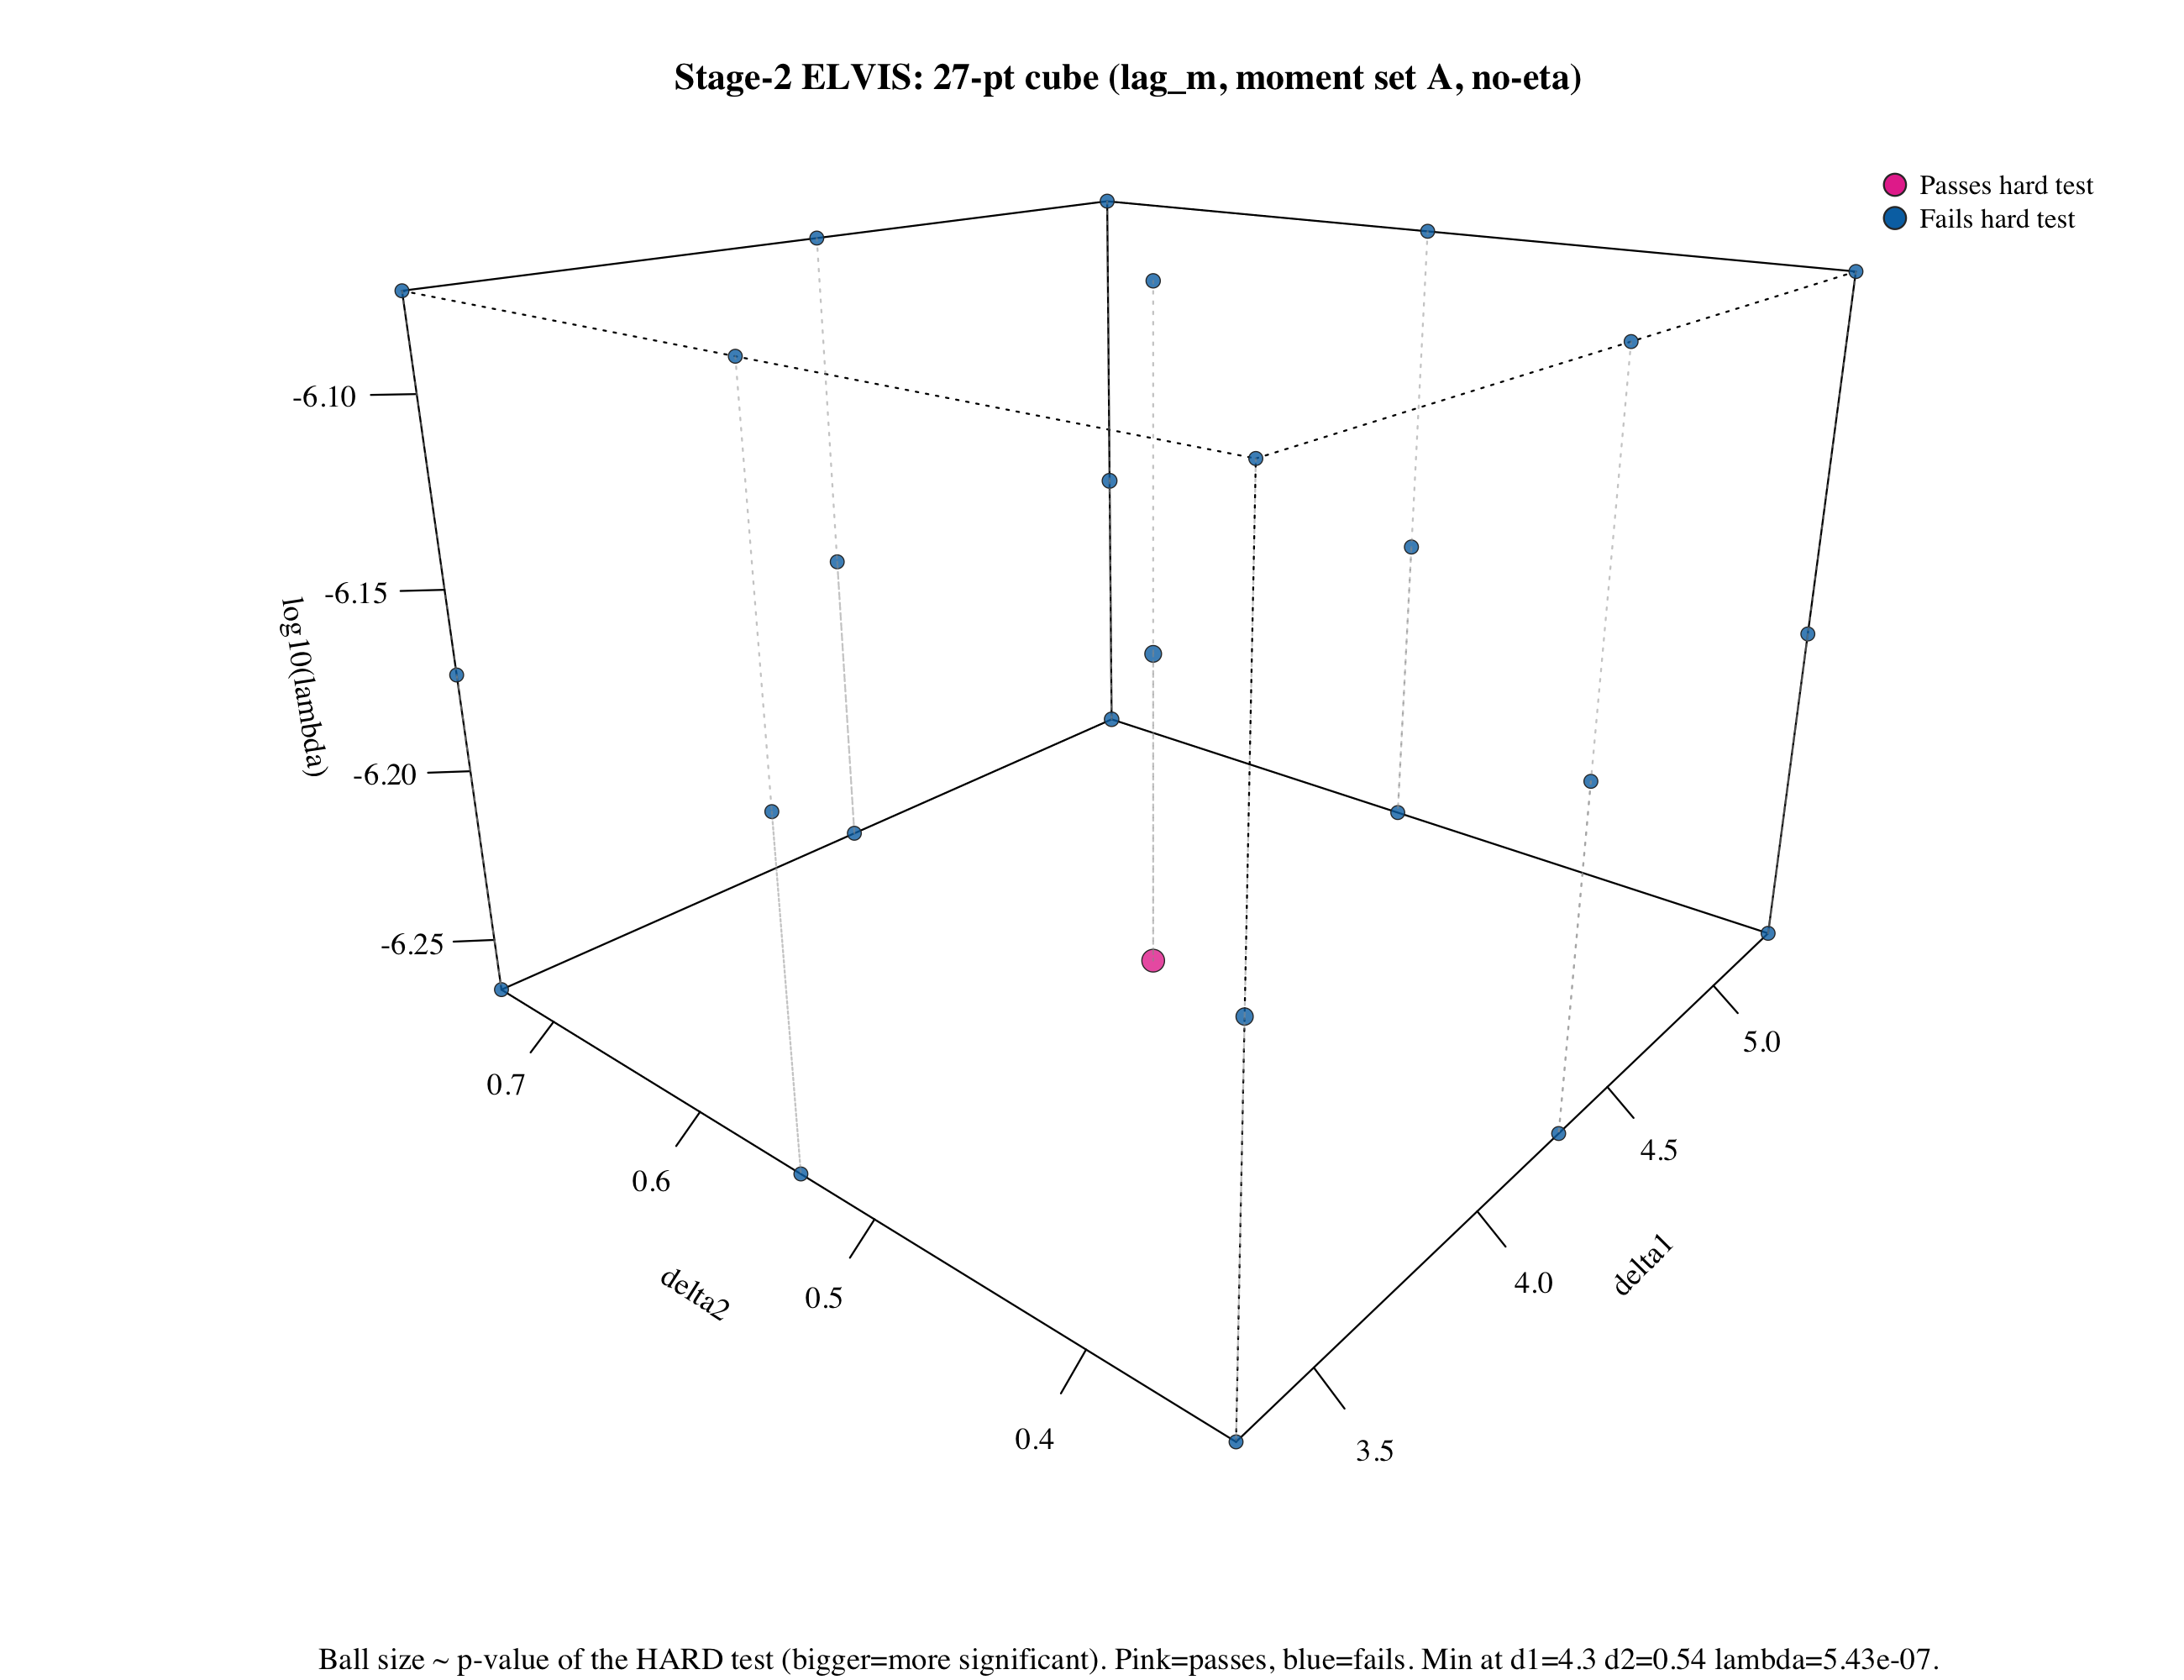
\includegraphics[width=\linewidth,height=0.85\textheight,keepaspectratio]{../Paper/images/1289-cube-lag_m-3d.png}
\end{center}
\end{frame}

\begin{frame}{Headline Estimates}
\protect\phantomsection\label{headline-estimates}
\begin{table}

\caption{\label{tbl-elvis-estimates}}

\centering{

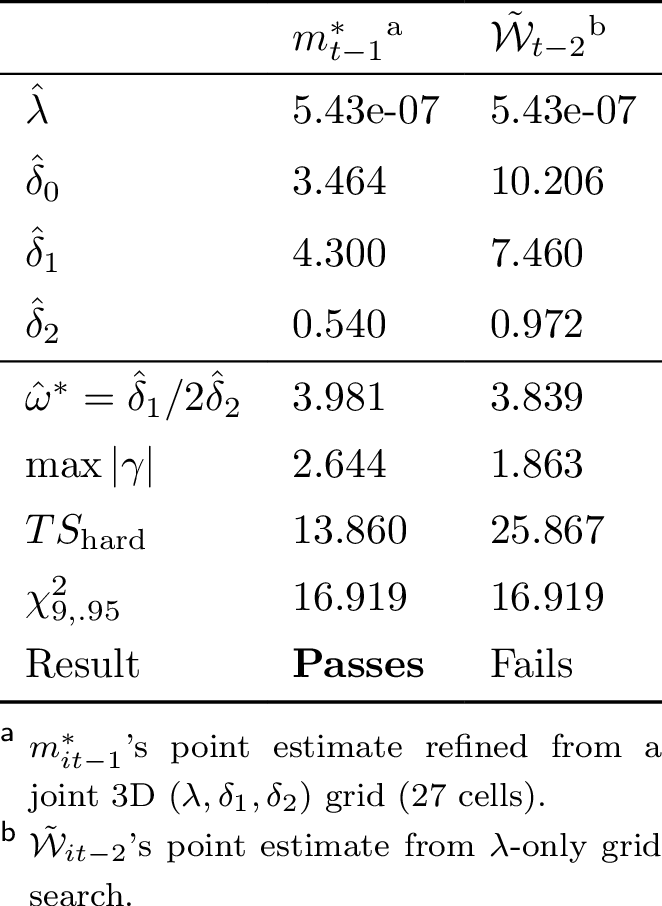
\includegraphics[width=\linewidth,height=0.8\textheight,keepaspectratio]{../Paper/tbls/1304-headline-estimates-table.png}

}

\end{table}%
\end{frame}

\begin{frame}{Interpreting the Estimates}
\protect\phantomsection\label{interpreting-the-estimates}
\begin{itemize}
\tightlist
\item
  Probabilities of detection are low, average audit-triggering threshold
  \(1/(2\hat\lambda)\approx\)\$920,000, while median reported materials
  \(\text{Med}[M^*]\approx\)\$8,414, the 95th percentile firms
  \$128,154, the 99th \$360,676, and the largest (trimmed) firm
  \$701,130
\item
  The cost function displays the expected U-shape, both
  \((\hat\delta_1,\hat\delta_2)\) display correct signs.

  \begin{itemize}
  \tightlist
  \item
    \(\hat\delta_1<0\) and \(\hat\delta_2>0\) the evasion cost function
    is decreasing in productivity up to \(\hat\omega^*\), then
    increasing again
  \item
    \(\hat\omega^*=3.98\) (\(m^*_{it-1}\)) and \(3.84\)
    (\(\tilde{\mathcal W}_{it-2}\)), the 86th (\(m^*_{it-1}\)) and 75th
    percentile (\(\tilde{\mathcal W}_{it-2}\)) (forward simulation)
  \end{itemize}
\end{itemize}
\end{frame}

\begin{frame}{How the Test Works}
\protect\phantomsection\label{how-the-test-works}
Test statistic at a candidate \(\theta\):
\(TS(\theta)=2n\hat L_n(\theta)\), profiled over \(\gamma\) (and any
nuisance parameters).

\begin{itemize}
\tightlist
\item
  Reported test: reject \(\theta\) if \(TS(\theta)>\chi^2_{d_g,.95}\)
  (\(d_g\) = number of moments) (\textbf{Theorem F.1}, Appendix F.
  Schennach 2014)
\end{itemize}
\end{frame}

\begin{frame}{What Detection Probability Does This Imply?}
\protect\phantomsection\label{what-detection-probability-does-this-imply}
\begin{columns}[T]
\begin{column}{0.3\linewidth}
\begin{itemize}
\tightlist
\item
  Mean \(\gg\) Median for both instruments; a right-skewed evasion
  distribution
\item
  P99 \(\to\) Max: detection probability jumps from 1-2\% at the 99th
  percentile, to \textasciitilde37\% for the most aggressive evader in
  the (0.5\%-trimmed) sample.
\item
  A handful of extreme evaders pull \(E[e]\) \textbf{up} \emph{and} the
  fitted \(\hat\lambda\) \textbf{down}
\end{itemize}
\end{column}

\begin{column}{0.7\linewidth}
\begin{table}

\caption{\label{tbl-prob-detection}}

\centering{

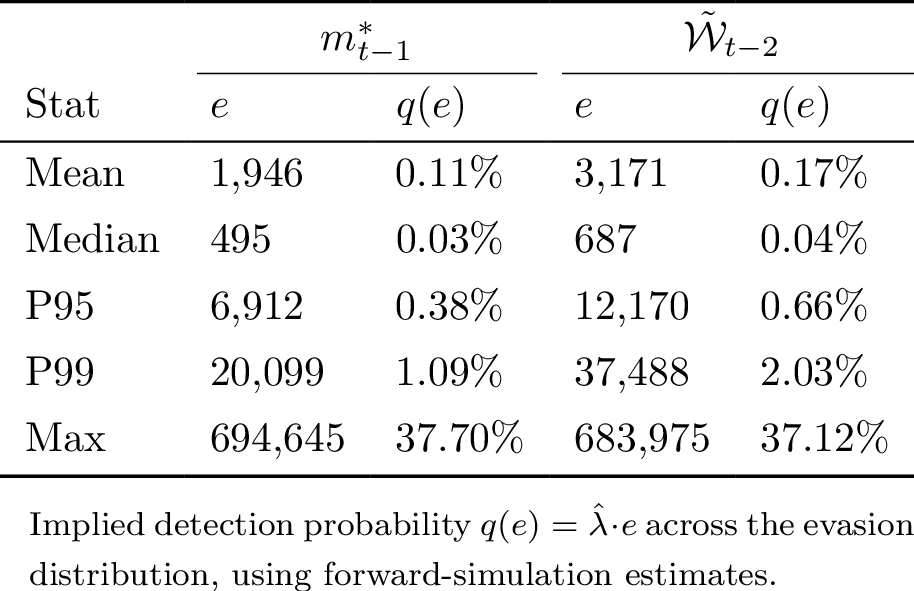
\includegraphics[width=\linewidth,height=0.7\textheight,keepaspectratio]{../Paper/tbls/1303-detection-prob-table.png}

}

\end{table}%
\end{column}
\end{columns}
\end{frame}

\begin{frame}{Trimming Sample}
\protect\phantomsection\label{trimming-sample}
Since few aggressive evaders were pushing the estimates of \(\lambda\)
down, I trimmed the sample at different percentiles of \(M^*\) to test
sensitivity of the estimates.

\begin{itemize}
\tightlist
\item
  At 0.5\% trim, \(\lambda\) seems to stabilize before jumping or start
  waving too much
\item
  \(\delta\)'s looked stable across the trim range, confirming that they
  were fitting the curvature of evasion, and lambda the level accross
  firms
\end{itemize}
\end{frame}

\begin{frame}{}
\protect\phantomsection\label{section}
\begin{center}
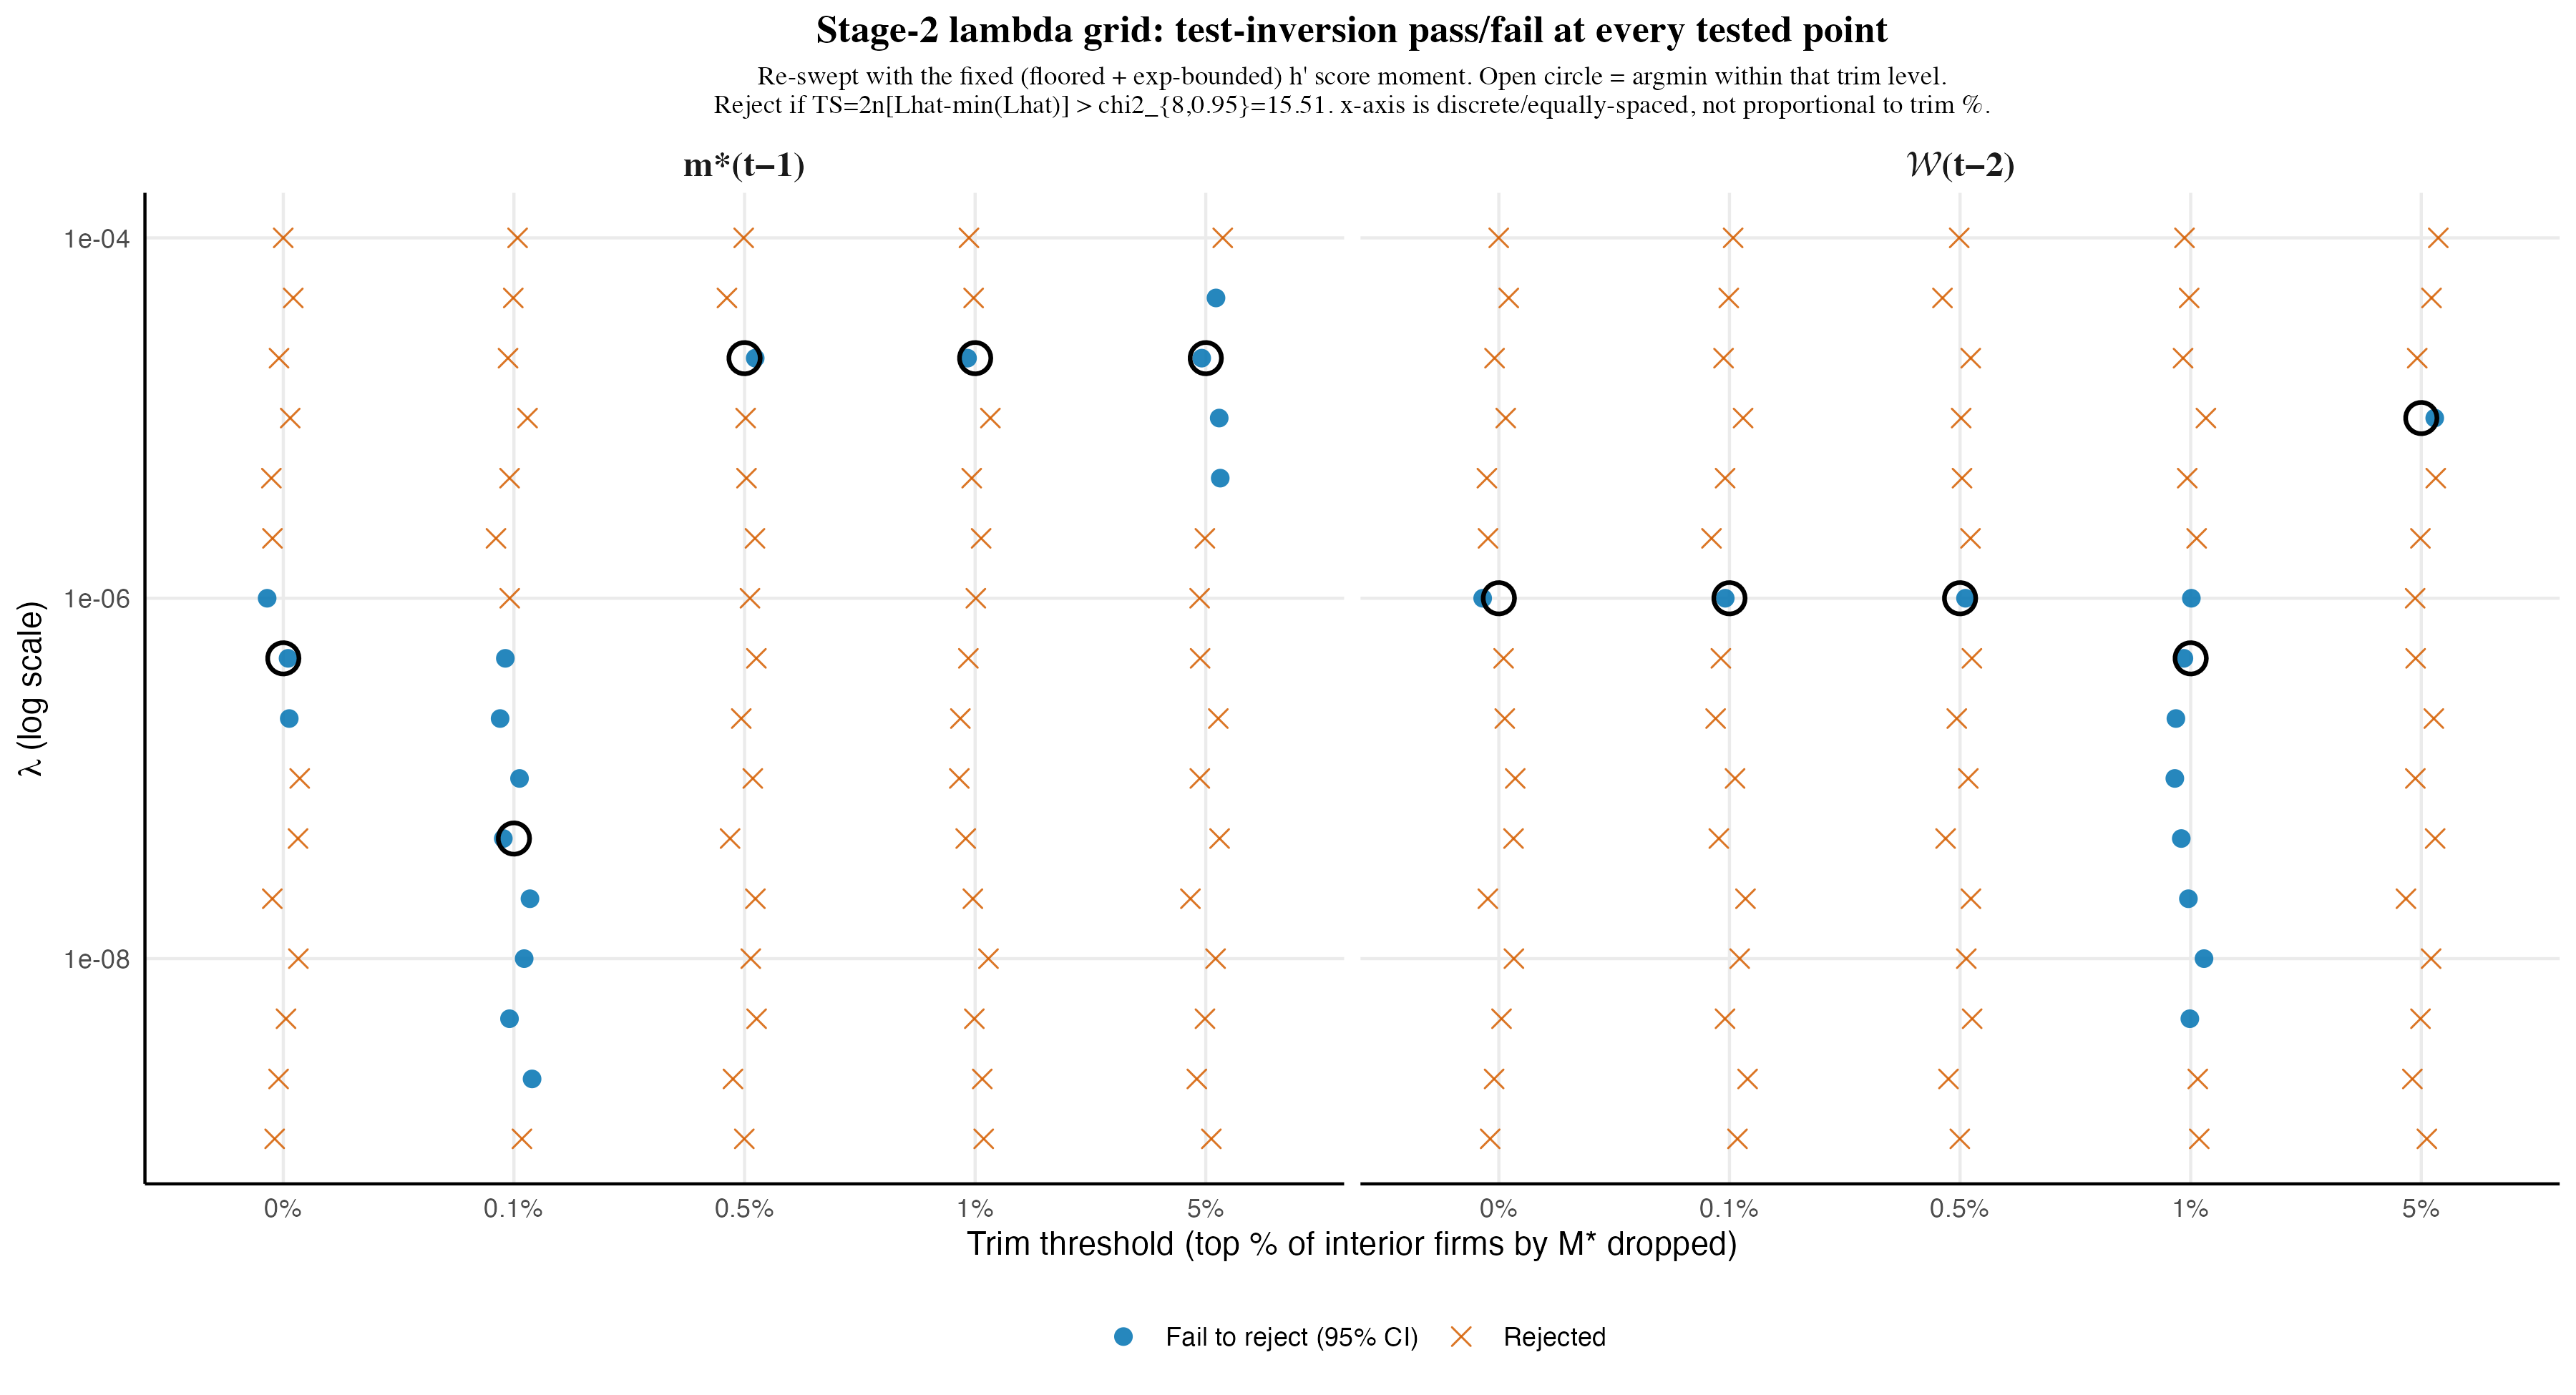
\includegraphics[width=\linewidth,height=0.9\textheight,keepaspectratio]{../Paper/images/1222-stage2-trim-all-gridpoints-refixed.png}
\end{center}
\end{frame}

\begin{frame}{Notes for Discussion}
\protect\phantomsection\label{notes-for-discussion}
\begin{itemize}
\tightlist
\item
\item
  \textbf{\(m^*_{it-1}\) is the instrument to lead with}: stable
  \(\hat\delta_1,\hat\delta_2\) across every search run so far, and the
  only instrument/grid combination to ever clear the conservative hard
  test
\item
  \textbf{\(\tilde{\mathcal W}_{it-2}\) confirms the same qualitative
  story but is the weaker instrument}: same U-shaped sign on
  \(\hat\delta_1,\hat\delta_2\), similar \(\hat\omega^*\), but doesn't
  clear the hard test at its own best point, and hasn't been run through
  the joint grid yet
\item
  \textbf{A first joint 3D grid is in (27 cells, coarse spacing)} ---
  not yet a full confidence region (only 1 tested cell clears the hard
  test), but real evidence for the fixed \(\hat\theta\) used in the
  counterfactual
\end{itemize}
\end{frame}

\begin{frame}{\(\lambda\) Search}
\protect\phantomsection\label{lambda-search}
\begin{itemize}
\tightlist
\item
  \(\lambda\) bounds derived directly from the data: the smallest
  \(\lambda\) for which not even the largest firm's evasion is ever
  constrained, up to the largest \(\lambda\) for which even the smallest
  firm is constrained

  \begin{itemize}
  \tightlist
  \item
    FOC: \(\lambda<\tfrac1{2e}\) aproximated with \(M^*=M+e\), assuming
    all is evasion, then the relevant range for \(\lambda\) is
    \([1/(2\max(M^*),1/(2\min(M^*))]\)
  \item
    During estimation, \(\lambda\) never hits the bounds
  \end{itemize}
\item
  16-point log-spaced grid (coarse pass, then a finer pass bracketing
  the region of interest)
\item
  \textbf{Sample}: 32,232 unincorporated firm-periods (3,340 at the
  \(\tau_P=0\) corner), top 0.5\% trimmed by \(M^*\); two
  productivity-instrument choices for \((\alpha_K,\alpha_L,\beta)\)
\end{itemize}
\end{frame}

\begin{frame}{}
\protect\phantomsection\label{section-1}
\end{frame}

\begin{frame}{\(\delta\) Search}
\protect\phantomsection\label{delta-search}
\end{frame}

\section{Laffer Curve (Counterfactual
Question)}\label{laffer-curve-counterfactual-question}

\begin{frame}[fragile]{Increasing Efficiency in the Counterfactual
Exercise}
\protect\phantomsection\label{increasing-efficiency-in-the-counterfactual-exercise}
Motivation and theoretical derivation:
\texttt{630-counterfactual-question.qmd}. Implementation:
\texttt{620-ELVIS.qmd}.

\footnotesize

\textbf{Goal:} use a control variate so the counterfactual test of
candidate revenue levels is more \emph{efficient} --- same target, less
noise.

\textbf{Why:} testing candidate revenue \(R\) against the data was
almost powerless. Revenue is dominated by \emph{firm size} --- large
firms pay vastly more sales tax than small ones --- and that size
variation has nothing to do with evasion. It's noise swamping the signal
we actually care about.

\textbf{How:} each firm's own sales tax paid, \(t1_i\), is fully
observed and predicts revenue almost perfectly (\(R^2\approx0.999\)).
Subtract off the size-driven, predictable part of revenue before testing
--- the classic control-variate variance-reduction technique (Hendry
1984), the same logic behind ANCOVA / CUPED adjustment in modern
experiments.

\textbf{Interpretation:} the estimator stays \textbf{consistent and
unbiased for the same expected revenue} \(E[R_i(\Delta)]\) --- nothing
about what a candidate \(R\) means, or how to read a confidence
interval, changes. The correction only strips out noise the estimator
didn't need; the same population quantity is estimated \textbf{more
efficiently} --- a tighter interval around the same target, not a
different one.
\end{frame}

\begin{frame}{Control-Variate Moment --- Details}
\protect\phantomsection\label{control-variate-moment-details}
\[g_{R,i}^{\text{adj}} = \Big[\frac{R_i(\Delta)}{pgdp_i}-\hat\beta\,\frac{t1_i}{pgdp_i}\Big] - \big[R-\hat\beta\,\mu_c\big]\]

\begin{itemize}
\tightlist
\item
  \(\hat\beta=0.9988\) (OLS, pooled across tested \(\Delta\)'s),
  \(\mu_c=E[t1_i/pgdp_i]\) --- both fixed, precomputed constants, never
  new \((\theta,\gamma)\) decision variables
\item
  \(E[g^{\text{adj}}_{R,i}]=E[g_{R,i}]\) exactly for \emph{any}
  \(\hat\beta\) --- verified to 6+ sig figs numerically, not just
  algebraically
\item
  Beats industry\(\times\)year TWFE decisively (38-41x vs.~2.5x), zero
  added dimensions, no small-cell risk (100/318 TWFE cells have \(<30\)
  obs)
\end{itemize}
\end{frame}

\begin{frame}{Testing the Laffer Curve}
\protect\phantomsection\label{testing-the-laffer-curve}
\begin{center}
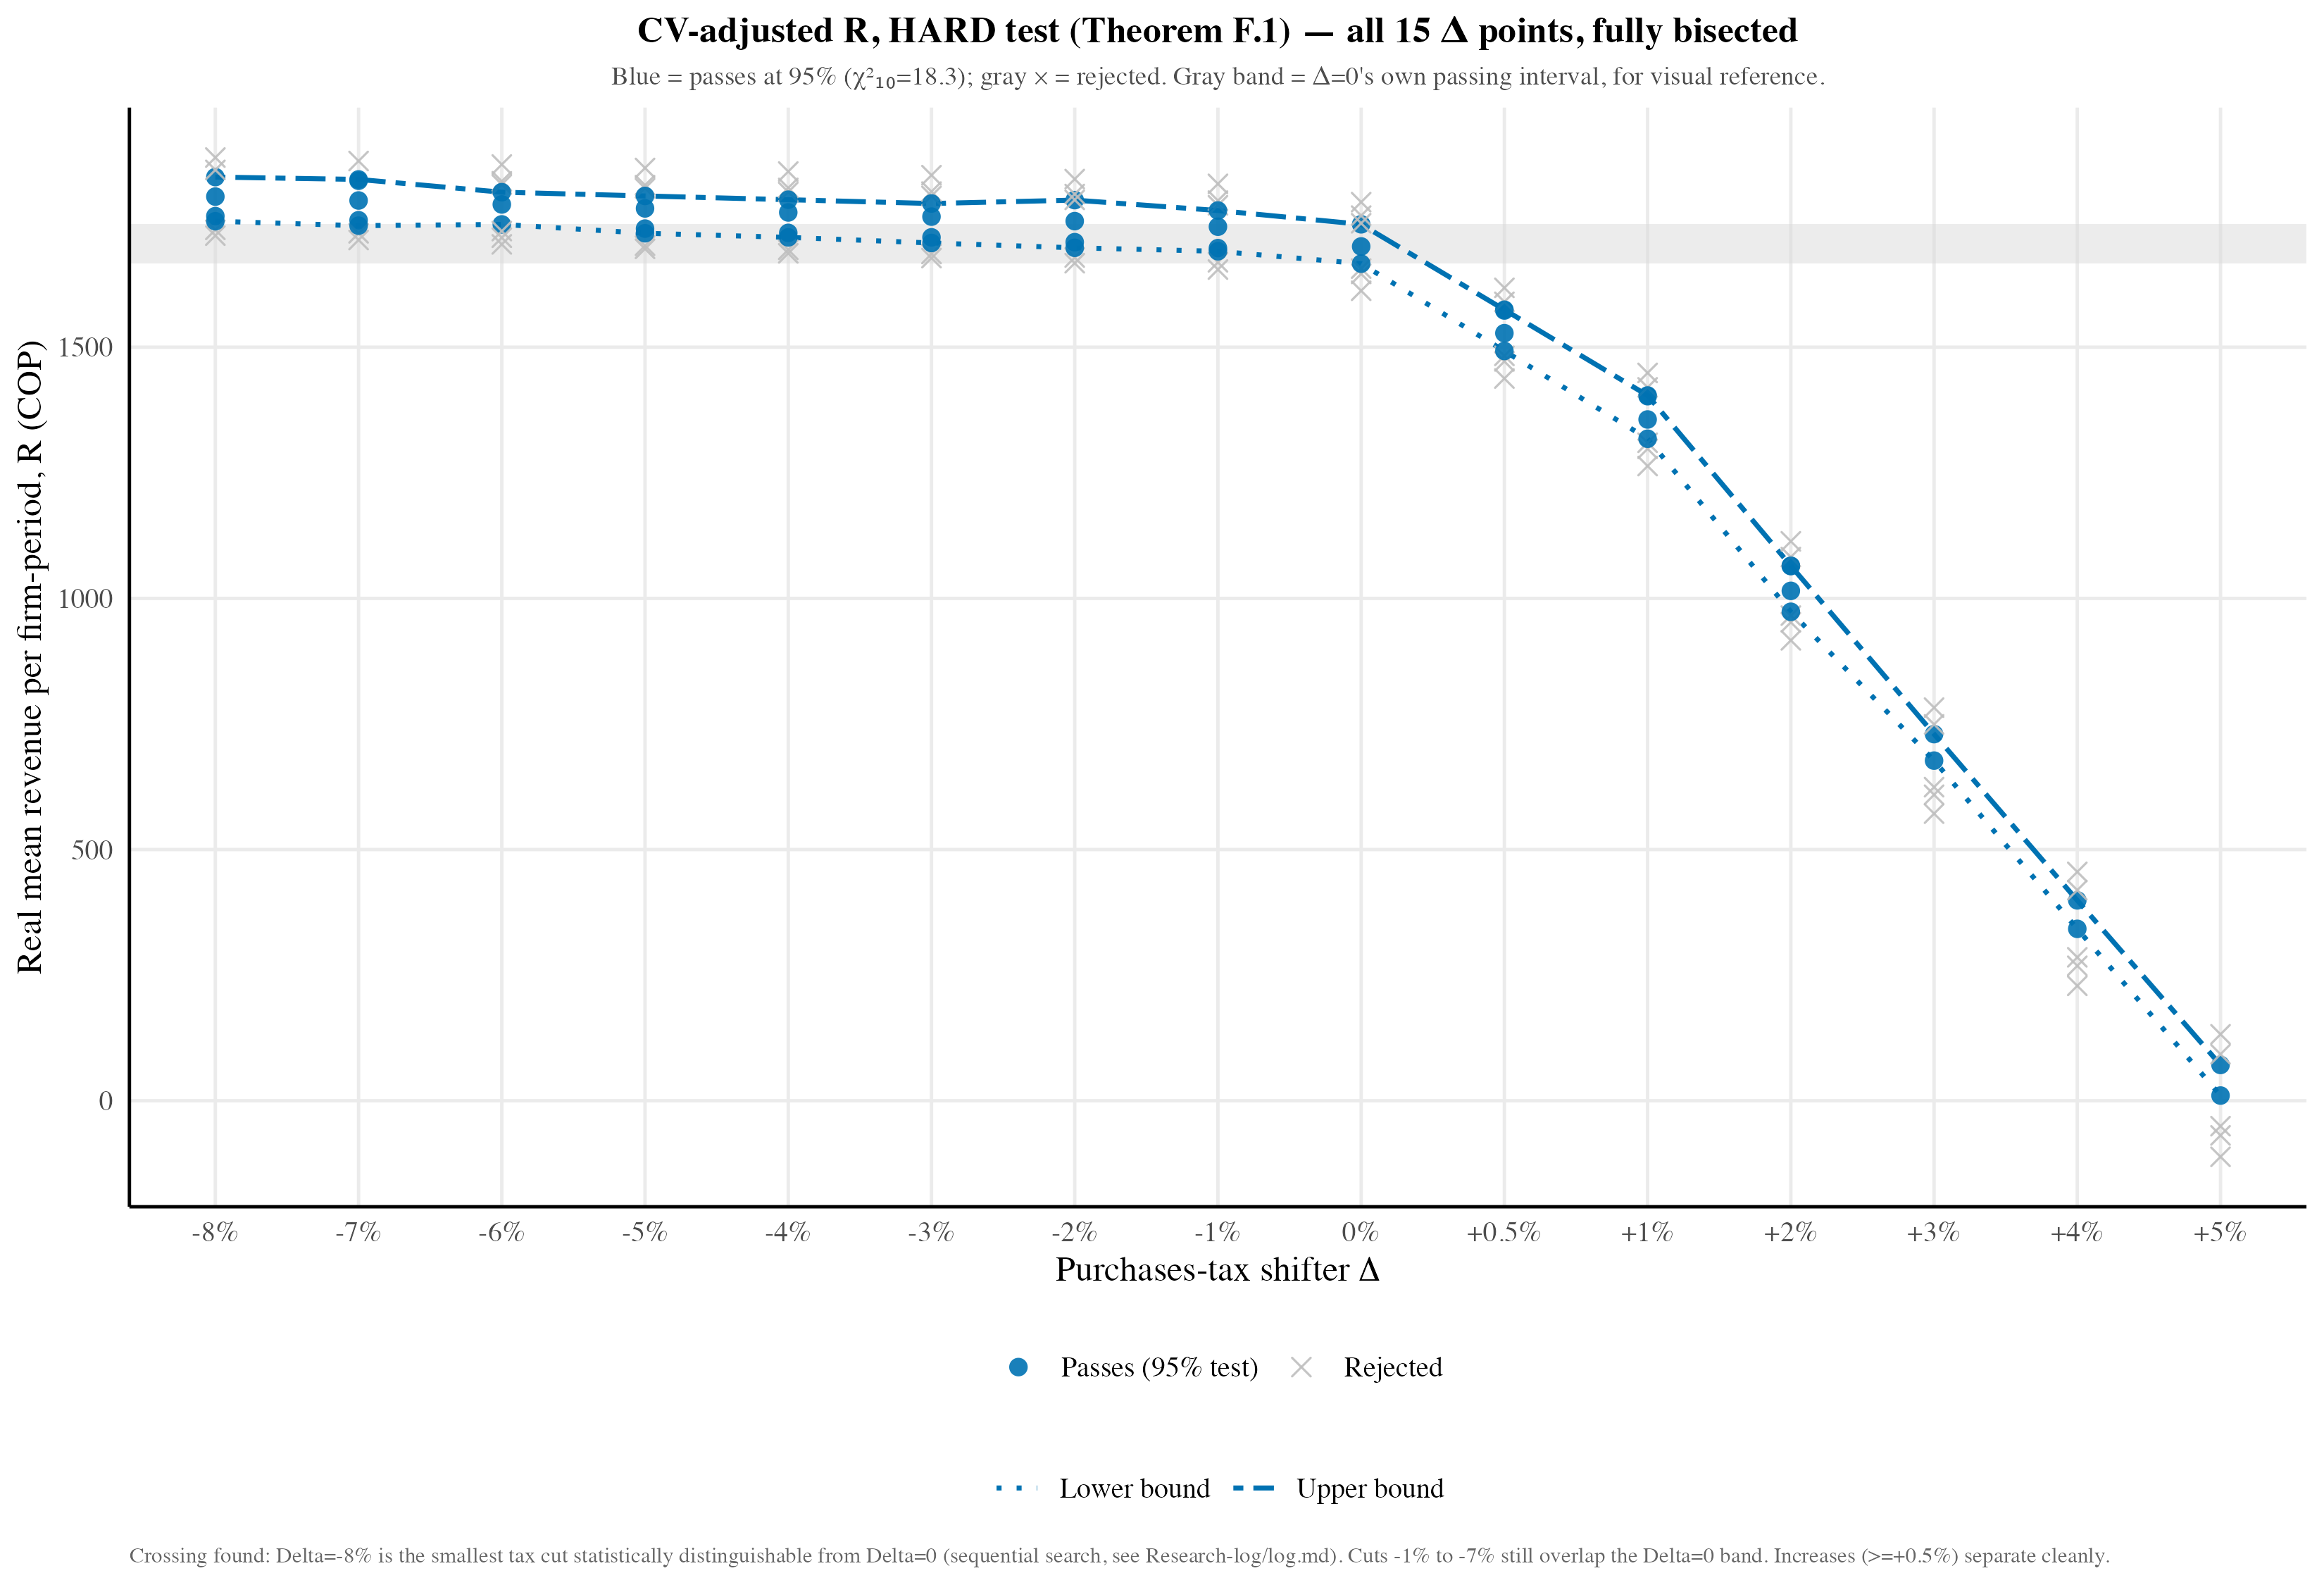
\includegraphics[width=\linewidth,height=0.78\textheight,keepaspectratio]{../Paper/images/1300-cv-15delta-hard.png}
\end{center}

Every point is a real candidate revenue level, tested against the data
(95\% confidence, gray band = current policy's own interval)
\end{frame}

\begin{frame}{Headline Result}
\protect\phantomsection\label{headline-result}
\begin{itemize}
\tightlist
\item
  A tax \textbf{increase} is bad news almost immediately: even a
  \textbf{0.5\% increase} is already statistically distinguishable from
  current policy
\item
  A tax \textbf{cut} helps too, but the gain only becomes statistically
  distinguishable once the cut reaches about \textbf{8\%} --- much
  larger than intuition suggests
\item
  Both results come from a formal statistical test, not a point estimate
\end{itemize}

\begin{center}
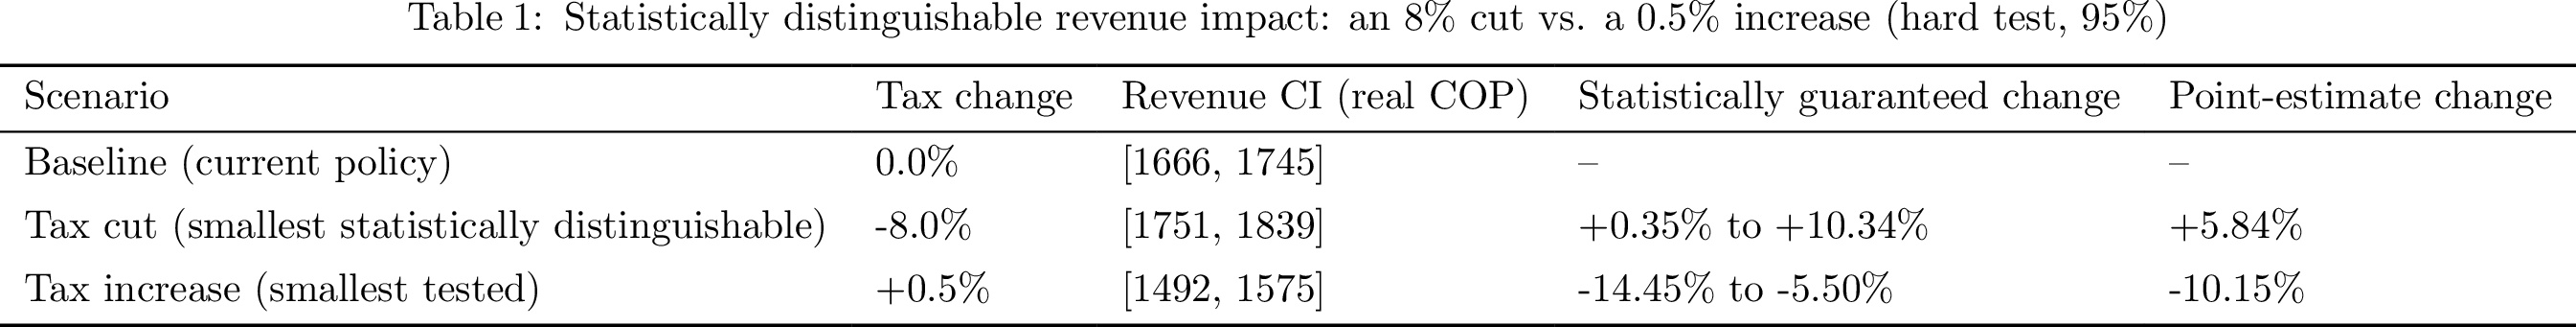
\includegraphics[width=\linewidth,height=0.3\textheight,keepaspectratio]{../Paper/tbls/1301-headline-pct-table.png}
\end{center}
\end{frame}

\begin{frame}{Why}
\protect\phantomsection\label{why}
Linear \(q\) + linear \(\kappa\) \(\Rightarrow\) new evasion is exactly
linear in the firm's own baseline evasion, with an intercept identical
across every firm:
\[\tilde e(\Delta)=\frac{e_i+\Delta/(2\lambda)}{1+\Delta}\]

Whether this looks like \emph{everyone moves together} or
\emph{heterogeneous, firm-by-firm} is a horse race between \(e_i\) and
\(\Delta/(2\lambda)\). Enforcement is estimated to be weak
(\(\hat\lambda\) tiny), so \(\Delta/(2\lambda)\) wins: a tax increase
shifts every firm by roughly the same large amount, while a cut removes
evasion firm-by-firm --- small evaders reach zero first, so the
aggregate response is gradual instead of a jump.
\end{frame}

\section{Estimating Tax Evasion by
Deconvolution}\label{estimating-tax-evasion-by-deconvolution}

\begin{frame}{Objective}
\protect\phantomsection\label{objective}
\begin{itemize}
\tightlist
\item
  Empirical exercise to motivate structural model
\end{itemize}
\end{frame}

\begin{frame}{What can be deconvoled and what can't}
\protect\phantomsection\label{sec-what-can-deconv}
\begin{tcolorbox}[enhanced jigsaw, arc=.35mm, bottomrule=.15mm, bottomtitle=1mm, breakable, colback=white, colbacktitle=quarto-callout-note-color!10!white, colframe=quarto-callout-note-color-frame, coltitle=black, left=2mm, leftrule=.75mm, opacityback=0, opacitybacktitle=0.6, rightrule=.15mm, title={Convolution (Meister, 2009)}, titlerule=0mm, toprule=.15mm, toptitle=1mm]

The density of the sum of two \textbf{independent} random variables is
equal to the \textbf{convolution} of the densities of both addends;
hence

\[
f_V = \int f_\varepsilon(V - u)f_u(u)du
\]

\end{tcolorbox}

Under \(\varepsilon \ind M, e\) and \(e \ind M\), with known
\(f_\varepsilon\) and \(u=\ln\left(\frac{M+e}{M}\right)\). Also
\(M^*=M+e\), and \(V=u+\varepsilon\).

Then, I can deconvolve:

\begin{itemize}
\tightlist
\item
  \(f_u\): \(f_V = \int f_\varepsilon(V - u)f_u(u)du\)
\end{itemize}
\end{frame}

\begin{frame}{I don't need \(f_e\), actually}
\protect\phantomsection\label{i-dont-need-f_e-actually}
What deconvolution recovers is the \textbf{overreporting log-ratio},
\(u_{it}\equiv\ln\left(\frac{M^*_{it}}{M_{it}}\right)=\ln\left(1+\frac{e_{it}}{M_{it}}\right)\),

\begin{itemize}
\tightlist
\item
  the \emph{share of overreported over true inputs}
\item
  the same object discussed previously, now given an explicit structural
  interpretation
\item
  Since it's a ratio, it's adjusted by the firm's true materials level
  and hence informative about the intensity of tax evasion
\item
  Had I recovered \(e\), I would have to normalize somehow to compare
  firms of different levels of material utilization
\end{itemize}

\footlineextra{\hyperlink{sec-denisities-plot}{Plotting \(\mathcal{V}\)
and \(\varepsilon\) \(\hookrightarrow\)}}
\end{frame}

\begin{frame}{Getting rid of the log}
\protect\phantomsection\label{getting-rid-of-the-log}
If I'm interested in only the density of the ratio, I can use a
\textbf{density transformation}

\textbf{Theorem 1.7.1 (Hogg et al. 2019)}: Let \(X\) be a continuous
random variable with pdf \(f_X(x)\) and support \(\mathbfcal{S}_X\). Let
\(Y=g(X)\) where \(g(x)\) is a one-to-one \emph{{[}monotonic{]}
differentiable} function on the support of \(X\), \(\mathbfcal{S}_X\).
Denote the inverse of \(g\) by \(x=g^{-1}(y)\) and
\(dx/dy=d[g^{-1}(y)]/dy\). Then, the pdf of \(Y\) is given by

\[
  f_Y(y)=f_X(g^{-1}(y))\Bigg|\frac{dx}{dy}\Bigg|, \text{for } y\in \mathbfcal{S}_Y
\]

where the support of \(Y\) is the set
\(\mathbfcal{S}_Y=\{y=g(x):x\in\mathbfcal{S}_X\}\)
\end{frame}

\begin{frame}{Getting density of the ratio}
\protect\phantomsection\label{getting-density-of-the-ratio}
Therefore, with \(X=u\) and \(g^{-1}(y)=\ln (1+y)\)

\begin{equation}\protect\phantomsection\label{eq-ratio-dens}{
f_{\frac eM}(y)= f_u\big(\ln (1+y)\big)\Bigg|\frac{1}{1+y}\Bigg|
}\end{equation}
\end{frame}

\begin{frame}{Informal proof}
\protect\phantomsection\label{informal-proof}
If \(U = g(R)\) for a strictly monotonic differentiable \(g\), then
\(f_R(r) = f_U(g(r))|g'(r)|\)

\textbf{Proof (via CDFs).} Take \(g\) strictly increasing (your case).
Then \[
F_R(r) = P(R\le r) = P\big(g(R)\le g(r)\big) = P(U\le g(r)) = F_U(g(r)),
\]

using that \(g\) increasing preserves the inequality direction.

Differentiate both sides in \(r\): \[
f_R(r) = \frac{d}{dr}F_U(g(r)) = f_U(g(r))g'(r).
\]

If \(g\) were decreasing instead, the inequality flips
(\(P(U\ge g(r))=1-F_U(g(r))\)), and differentiating introduces a minus
sign that exactly cancels the sign of \(g'(r)\), hence \(|g'(r)|\) of
the general formula.

Everything goes through unchanged conditional on \(Z=z\) \sm{(just work
with \(F_{R|Z}(\cdot\mid z)\), \(F_{u|Z}(\cdot\mid z)\) throughout).}
\end{frame}

\begin{frame}{Discussion}
\protect\phantomsection\label{discussion-1}
Deconvolution estimates the unconditional \(f_u\) because of how we set
it up

\begin{itemize}
\tightlist
\item
  From \(f_u\), we can learn the probability of a firm of overreporting
  \(u\), \(P(U<u)=\int_0^uf_u(t)dt\), or

  \begin{itemize}
  \tightlist
  \item
    the expected overreportig \(\mu_u=\int u f_u(u)du\)
  \end{itemize}
\item
  This is the uncoditional probability, the same for all firms
  regardless of their characteristics
\item
  We might be interested in the \emph{probability of overreporting
  conditional} on the firm size
\end{itemize}
\end{frame}

\begin{frame}{What if we are interested in the conditional density?}
\protect\phantomsection\label{what-if-we-are-interested-in-the-conditional-density}
\[
\begin{aligned}
    f_{V|Z}(V\mid Z)&=\frac{f_{V,Z}(V,Z)}{f_Z(Z)}\\
    &=\int f_{V|u,Z}(V\mid u,Z)\,f_{u|Z}(u\mid Z)\,du\\
    &=\int f_\varepsilon(V-u)\,f_{u|Z}(u\mid Z)\,du
\end{aligned}
\]

using

\begin{itemize}
\tightlist
\item
  \(f_{V|u,Z}(V\mid u,Z)=f_{\varepsilon|u,Z}(V-u\mid u,Z)\) ---
  \(V=u+\varepsilon\) conditional on \(u\)
\item
  \(\varepsilon\perp(u,Z)\) \textbf{jointly}, so
  \(f_{\varepsilon|u,Z}=f_\varepsilon\)
\end{itemize}

with \(u\not\ind Z\) (otherwise conditioning on \(Z\) would be
pointless).
\end{frame}

\begin{frame}{Estimating the Conditional distribution}
\protect\phantomsection\label{sec-estimating-cond-deconv}
\begin{itemize}
\tightlist
\item
  \textbf{Discrete/bucketed \(Z\)} (e.g.~quintiles of \(K_{it}\) or
  \(L_{it}\)): the same 1-D deconvolution separately within each bucket.

  \begin{itemize}
  \tightlist
  \item
    We've already looked into \(E[u|Z]\)
  \end{itemize}
\item
  \textbf{Continuous \(Z\)}: nonparametric deconvolution with a
  continuous covariate

  \begin{itemize}
  \tightlist
  \item
    Literature: \(f_{u|V}(u|V)\) (Wang and Ye 2015), \(E[Z|u]\) (Fan and
    Truong 1993), and \(f_{Z|u}\) (Huang and Zhou 2020)
  \item
    \(f_{u|Z}\): feasible using
    \hyperlink{sec-cond-deconv-appendix}{characteristic functions and
    kernels}
  \end{itemize}
\item
  Ideally, what I want is \(f_{e|\omega}\), but that's what \(f_\psi\)
  is, the object I wil obtain with the structural approach
\end{itemize}
\end{frame}

\section{Conditional Deconvolution ---
Backup}\label{conditional-deconvolution-backup}

\begin{frame}{What About the Full Distribution?}
\protect\phantomsection\label{sec-cond-deconv-appendix}
\begin{itemize}
\item
  So far: \(E[u_{ijt}\mid Z_{ijt}]\), and only at 10 decile bins of
  \(Z\)
\item
  Natural next question: the whole conditional density
  \(f_{u\mid Z}(u\mid z)\), for \(Z\) continuous

  \begin{itemize}
  \tightlist
  \item
    Is the size gradient in the \emph{level} of evasion, its
    \emph{spread}, or its \emph{shape}?
  \end{itemize}
\end{itemize}
\end{frame}

\begin{frame}{Aside: How Deconvolution Works}
\protect\phantomsection\label{aside-how-deconvolution-works}
We never observe \(u_{ijt}\) directly --- only
\(V_{ijt}=u_{ijt}+\varepsilon_{ijt}\), a ``blurred'' version of it

\begin{itemize}
\item
  A histogram of \(V\) mixes the true shape of \(u\) with the noise
  \(\varepsilon\) --- the density of a sum of independent things is the
  \emph{convolution} of their densities, \(f_V=f_u * f_\varepsilon\)
\item
  Convolutions are hard to undo directly, but they become simple
  \emph{multiplication} after a Fourier transform (the characteristic
  function): \[
  \phi_V(t)=\phi_u(t)\,\phi_\varepsilon(t) \quad\Longrightarrow\quad \phi_u(t)=\frac{\phi_V(t)}{\phi_\varepsilon(t)}
  \]
\item
  Estimate \(\phi_V\) from the data, divide by the already-known
  \(\phi_\varepsilon\), transform back \(\to \hat f_u\)
\item
  This is exactly the (unconditional) trick behind the first-stage
  results (Carroll and Hall 1988; Stefanski and Carroll 1990)
\end{itemize}
\end{frame}

\begin{frame}{Conditional Version: Add a Local Window}
\protect\phantomsection\label{conditional-version-add-a-local-window}
Same trick, done separately for each value of \(Z\):

\begin{itemize}
\tightlist
\item
  Instead of using \emph{all} firms to build one blurred distribution,
  use only firms with \(Z_i\) close to \(z\) --- a moving local window,
  weighted by a kernel \(K\)
\item
  Un-blur \emph{that} local distribution the same way as before
\end{itemize}

\[
\begin{aligned}
\hat\phi_{V\mid Z=z}(t)&=\frac{\sum_i K\!\left(\frac{Z_i-z}{h}\right)e^{itV_i}}{\sum_i K\!\left(\frac{Z_i-z}{h}\right)}\\[4pt]
\;\;\Longrightarrow\;\;\hat f_{u\mid Z=z}(u)&=\frac{1}{2\pi}\int e^{-itu}\,\frac{\hat\phi_{V\mid Z=z}(t)}{\phi_\varepsilon(t)}\,\omega(t)\,dt
\end{aligned}
\]

\begin{itemize}
\tightlist
\item
  \(\omega(t)\): a damping weight, standard in any deconvolution, to
  keep the division numerically stable
\item
  Valid because \(\varepsilon\perp(u,Z)\): within any \(Z\)-window, the
  noise is still independent of \(u\) --- the same assumption used
  throughout this section
\end{itemize}
\end{frame}

\begin{frame}{Is This Standard?}
\protect\phantomsection\label{is-this-standard}
\begin{itemize}
\tightlist
\item
  (Fan and Truong 1993), already cited on the ``is it feasible?'' slide,
  addresses the \emph{mirror-image} problem: a noisy covariate and a
  clean outcome (see also (Huang and Zhou 2020) for the
  conditional-density version of that same direction)
\item
  Ours runs the other way --- clean \(Z\), noisy \(u\) --- which is why
  the conditional \emph{mean} never needed correcting:
  \(\varepsilon\perp Z \Rightarrow E[V\mid Z]=E[u\mid Z]\)
\item
  Only the \emph{density} needs deconvolving, and the tool is just the
  classical deconvolution kernel (Carroll and Hall 1988; Stefanski and
  Carroll 1990), applied inside a local window --- a natural
  combination, not (to our knowledge) a named result in the literature
\end{itemize}
\end{frame}

\begin{frame}{Do We Need the Full Density?}
\protect\phantomsection\label{do-we-need-the-full-density}
\begin{itemize}
\item
  The conditional mean already carries the headline story: evasion rises
  then falls with size --- going further only pays off if it answers a
  question the mean can't
\item
  The one moment that would matter: the conditional \textbf{variance}
  \(\mathrm{Var}(u\mid Z=z)\)

  \begin{itemize}
  \tightlist
  \item
    Does ``large firms don't evade'' mean (a) \emph{every} large firm
    individually evades a little --- tight distribution near zero, like
    the corporations --- or (b) a mix of some firms still evading
    heavily and others near zero that cancel out in the mean?
  \item
    \begin{enumerate}
    [(a)]
    \tightlist
    \item
      vs.~(b) is a real audit-targeting question: under (a), size alone
      is a good targeting rule at the top; under (b) it isn't --- some
      large firms are still hiding substantial evasion behind the
      average
    \end{enumerate}
  \end{itemize}
\item
  If pushed further: the full nonparametric conditional deconvolution
  (previous slides) is the general method; cumulant/method-of-moments
  matching is a cheap over-identification check on the variance
  estimate, not a substitute for it
\end{itemize}

\footlineextra{\hyperlink{sec-estimating-cond-deconv}{\(\hookleftarrow\)}}
\end{frame}

\section{Appendix}\label{appendix}

\begin{frame}{}
\protect\phantomsection\label{section-2}
\appendix
\end{frame}

\section{Naive MSM and MSL}\label{naive-msm-and-msl}

\begin{frame}{Recall: Two Identities From the Model}
\protect\phantomsection\label{recall-two-identities-from-the-model}
\begin{equation}\protect\phantomsection\label{eq-eva-emp}{
\mathcal{V}_{it} \equiv \ln\left(\frac{\rho_t M^*_{it}}{P_tY_{it}}\right)-\ln(\beta) = \ln\left(\frac{M^*_{it}}{M_{it}}\right)-\varepsilon_{it}
}\end{equation}

\begin{equation}\protect\phantomsection\label{eq-tilde-big-w}{
\tilde{\mathcal{W}}_{it}\equiv \mathcal{W}_{it}-\alpha_K k_{it}-\alpha_L l_{it}=\omega_{it}+(1-\beta)\varepsilon_{it}
}\end{equation}
\end{frame}

\begin{frame}{Solving for \(M\) and \(e\)}
\protect\phantomsection\label{solving-for-m-and-e}
\textbf{NEW} From Equation~\ref{eq-eva-emp}, I can \emph{algebraically
solve} for true inputs as function of observed variables and an the
error term,

\begin{itemize}
\tightlist
\item
  \(M_{it}=M^*_{it}\textbf{e}^{-\mathcal{V}_{it}-\varepsilon_{it}}\).
\end{itemize}

Therefore,

\[
\begin{aligned}
    e_{it}=&M^*_{it}-M_{it}\\
    =&M^*_{it}\left(1-\textbf{e}^{-\mathcal{V}_{it}-\varepsilon_{it}}\right)
\end{aligned}
\]

\begin{itemize}
\tightlist
\item
  \(\varepsilon_{it}\) is not observed firm-by-firm, only its
  distribution \(f_\varepsilon\)
\item
  not a literal point recovery of \(e_{it}\), but the map that could be
  evaluated for some draw of \(\varepsilon^{(s)}\sim\hat f_\varepsilon\)
\end{itemize}
\end{frame}

\begin{frame}{Recast in terms of one unobservable}
\protect\phantomsection\label{recast-in-terms-of-one-unobservable}
I can do the same and solve for \(\omega_{it}\) from
Equation~\ref{eq-tilde-big-w}

For each value of \(\varepsilon\) everything else is pinned down:

\begin{equation}\protect\phantomsection\label{eq-e-eps}{
e_{it}(\varepsilon)=M^*_{it}\big(1-\textbf{e}^{-\mathcal V_{it}-\varepsilon}\big)
}\end{equation}

\begin{equation}\protect\phantomsection\label{eq-w-eps}{
\omega_{it}(\varepsilon)=\tilde{\mathcal W}_{it}-(1-\beta)\varepsilon
}\end{equation}

\begin{equation}\protect\phantomsection\label{eq-psi-eps}{
\psi_{it}(\varepsilon)=h\big(e_{it}(\varepsilon)\big)-\delta_0+\delta_1\,\omega_{it}(\varepsilon)-\delta_2\omega_{it}(\varepsilon)^2
}\end{equation}
\end{frame}

\begin{frame}{Drawing from \(f_\varepsilon\)}
\protect\phantomsection\label{drawing-from-f_varepsilon}
Substituting Equation~\ref{eq-e-eps} and Equation~\ref{eq-w-eps} into
Equation~\ref{eq-psi-eps}, and simplifying

\begin{equation}\protect\phantomsection\label{eq-psi-mom}{
\begin{aligned}
    \psi_{it}+&\delta_1(1-\beta)\varepsilon=\\
    &\ln(\tau\rho_t)+\ln(1-2\lambda M^*_{it}(1-\textbf{e}^{-\mathcal{V}_{it}-\varepsilon}))\\
    &-\delta_0+2\delta_2(1-\beta)\tilde{\mathcal{W}}_{it}\varepsilon-\delta_2(1-\beta)^2\varepsilon^2\\
    &+\delta_1 \tilde{\mathcal{W}}_{it}-\delta_2\tilde{\mathcal{W}}_{it}^2
\end{aligned}
}\end{equation}
\end{frame}

\begin{frame}{Taking conditional expectation}
\protect\phantomsection\label{taking-conditional-expectation}
Assuming \(\psi\perp Z\), \(\varepsilon\perp Z\), and
\(\omega\perp\varepsilon\).
\(\varepsilon\perp Z\Rightarrow E[\delta_1(1-\beta)\varepsilon\mid Z]=\delta_1(1-\beta)E[\varepsilon\mid Z]=0\)

\begin{equation}\protect\phantomsection\label{eq-psi-mom-exp}{
\begin{aligned}
    0=&\ln(\tau\rho_t)+E[\ln(1-2\lambda M^*_{it}(1-\textbf{e}^{-\mathcal{V}_{it}-\varepsilon}))|Z]\\
    &\underbrace{-\delta_0-\delta_2(1-\beta)^2\sigma_\varepsilon^2}_{\textit{Constant (known from stage 1)}}\\
    &+\delta_1 \tilde{\mathcal{W}}_{it}-\delta_2\tilde{\mathcal{W}}_{it}^2
\end{aligned}
}\end{equation}
\end{frame}

\begin{frame}{Why not simulated GMM with instruments?}
\protect\phantomsection\label{why-not-simulated-gmm-with-instruments}
Everything in Equation~\ref{eq-psi-mom-exp} is data and parameters,
\textbf{except}: \[
\begin{aligned}
    \ell_{it}(\varepsilon;\lambda)\equiv&\ln\!\big(1-2\lambda M^*_{it}(1-\textbf{e}^{-\mathcal V_{it}-\varepsilon})\big)\\
    &=\ln\!\big(1-2\lambda M^*_{it}\big(1-\textbf{e}^{-\ln\left(\frac{M^*_{it}}{M_{it}}\right)+\varepsilon_{it}-\varepsilon^{(s)}}\big)\big)\\
    &=\ln\!\big(1-2\lambda \underbrace{\left(M^*_{it}-M_{it}\textbf{e}^{\varepsilon_{it}-\varepsilon^{(s)}}\right)}_{\ne e_{it}}\big)\\
\end{aligned}
\]

The moment to holds under \(\varepsilon_{it}\), the realized measurement
error for firm \(it\), \(\ell_{it}(\varepsilon_{it};\lambda)\)
\end{frame}

\begin{frame}{Simulating the nonlinear term}
\protect\phantomsection\label{simulating-the-nonlinear-term}
If we hold firm \(it\)'s own \((M^*_{it},\mathcal V_{it})\) fixed and
simulate \(\varepsilon\), \[
\hat\ell_{it}^S(\lambda)=\frac1S\sum_{s=1}^S\ell_{it}(\varepsilon^{(s)};\lambda),\qquad \varepsilon^{(s)}\stackrel{iid}{\sim}\hat f_\varepsilon
\]

By the LLN, as \(S\to\infty\):
\(\hat\ell_{it}^S(\lambda)\xrightarrow{a.s.}\bar\ell_{it}(\lambda)\equiv\int\ell_{it}(\varepsilon;\lambda)\,f_\varepsilon(\varepsilon)\,d\varepsilon\)

In general, however,

\[
\bar\ell_{it}(\lambda)\ne\ell_{it}(\varepsilon_{it};\lambda)
\]
\end{frame}

\begin{frame}{Why \(\mathcal V_{it}\) already contains
\(\tilde{\mathcal W}_{it}\)}
\protect\phantomsection\label{why-mathcal-v_it-already-contains-tildemathcal-w_it}
At the truth (\(\varepsilon=\varepsilon_{it}\)), \(e_{it}\) solves the
firm's FOC: \(e_{it}=e^*(\psi_{it},\omega_{it})\) (inverting
Equation~\ref{eq-psi-eps} for \(e\)).

Substitute this and Equation~\ref{eq-w-eps} into
Equation~\ref{eq-e-eps}'s own inverse,
\(\mathcal V_{it}=\ln\big(M_{it}+e_{it}/(M_{it})\big)-\varepsilon_{it}\):

\[
\mathcal V_{it}=\ln\!\left(\frac{M_{it}+e^*\big(\psi_{it},\,\tilde{\mathcal W}_{it}-(1-\beta)\varepsilon_{it}\big)}{M_{it}}\right)-\varepsilon_{it}
\]

\begin{itemize}
\tightlist
\item
  \(\varepsilon_{it}\) must be consistent with \(\mathcal V_{it}\) and
  \(\tilde{\mathcal W}_{it}\) jointly
\item
  \(\ell_{it}\) must be conditioned on
  \((\mathcal V_{it},\tilde{\mathcal W}_{it})\)
\end{itemize}
\end{frame}

\begin{frame}{The conditional expectation}
\protect\phantomsection\label{the-conditional-expectation}
Since \(\mathcal V_{it}\) depends on \(\tilde{\mathcal W}_{it}\) too
(shown above), condition on both, then apply the law of iterated
expectations:

\[
E[\ell_{it}(\varepsilon_{it};\lambda)\mid Z]=E\Big[E[\ell_{it}(\varepsilon_{it};\lambda)\mid Z,\mathcal V_{it},\tilde{\mathcal W}_{it}]\ \Big|\ Z\Big]
\]

\[
E[\ell_{it}(\varepsilon_{it};\lambda)\mid Z,\mathcal V_{it},\tilde{\mathcal W}_{it}]=\int \ell_{it}(\varepsilon;\lambda)\,f_{\varepsilon\mid \mathcal V_{it},\tilde{\mathcal W}_{it},Z}(\varepsilon)\,d\varepsilon
\]

\begin{itemize}
\tightlist
\item
  LIE reveals the inner integral needs
  \(f_{\varepsilon\mid\mathcal V_{it},\tilde{\mathcal W}_{it},Z}\), the
  density of \(\varepsilon\) \textbf{conditional on this firm's own
  \(\mathcal V_{it}\)}
\item
  \(\hat\ell_{it}^S(\lambda)\) instead integrates against the
  \textbf{unconditional} \(f_\varepsilon\)
\item
  Since \(\mathcal V_{it}=u_{it}-\varepsilon_{it}\) by construction
  \(\varepsilon_{it}\not\ind\mathcal V_{it}\)
\end{itemize}
\end{frame}

\begin{frame}{Testing with data}
\protect\phantomsection\label{testing-with-data}
I simulate \(\varepsilon^{(s)}\), S=250, from \(\hat{f_{\varepsilon}}\),
efficient GMM objective weigthed by \(\hat\Omega^{-1}\), and test the
J-statistic against its \(\chi^2\) distribution (Hansen 1982)

\(\varepsilon^{(s)}\) drawn from CORP firms' empirical distribution,
feasibility-filtered (\(e>0,M>0\));

Two set of moment conditions tested:

\begin{itemize}
\tightlist
\item
  Exactly identified (\(d_g=d_{\theta}=4\)):
  \(g(\theta)=(\psi,\psi\omega,\psi\omega^2,\varepsilon h')\) (last
  moment is a score term for \(\lambda\)). I report the value of the
  objective function.
\item
  Overidentified (\(d_g=5>d_{\theta}=4\)): 5th moment added,
  \(\psi\ln M\). I report value of obj. fun and J-statistical test
\end{itemize}
\end{frame}

\begin{frame}{Results of the test}
\protect\phantomsection\label{results-of-the-test}
{\def\LTcaptype{none} % do not increment counter
\begin{longtable}[]{@{}
  >{\raggedright\arraybackslash}p{(\linewidth - 8\tabcolsep) * \real{0.2000}}
  >{\raggedright\arraybackslash}p{(\linewidth - 8\tabcolsep) * \real{0.2000}}
  >{\raggedright\arraybackslash}p{(\linewidth - 8\tabcolsep) * \real{0.2000}}
  >{\raggedright\arraybackslash}p{(\linewidth - 8\tabcolsep) * \real{0.2000}}
  >{\raggedright\arraybackslash}p{(\linewidth - 8\tabcolsep) * \real{0.2000}}@{}}
\toprule\noalign{}
\begin{minipage}[b]{\linewidth}\raggedright
\end{minipage} & \begin{minipage}[b]{\linewidth}\raggedright
\(\hat L_n\) (\(d_g=4\))
\end{minipage} & \begin{minipage}[b]{\linewidth}\raggedright
\(\hat L_n\) (\(d_g=5\))
\end{minipage} & \begin{minipage}[b]{\linewidth}\raggedright
\(J\)
\end{minipage} & \begin{minipage}[b]{\linewidth}\raggedright
\(\chi^2_{1,.95}\)
\end{minipage} \\
\midrule\noalign{}
\endhead
\(m^*_{it-1}\) & 1.022 & 1.020 & 29,258 & 3.84 \\
\(\tilde{\mathcal{W}}_{it-2}\) & 1.011 & 1.009 & 28,961 & 3.84 \\
\bottomrule\noalign{}
\end{longtable}
}

\begin{itemize}
\tightlist
\item
  Exactly identified: \(\hat L_n\) not close to zero, parameter
  estimates hit generous bounds
\item
  Overidentified: Under the null, \(H_0: g(\theta)=0\). Rejects null at
  95\% by a large factor. \(\hat L_n\) still not below 1.
\end{itemize}
\end{frame}

\begin{frame}{Fitted Parameters}
\protect\phantomsection\label{fitted-parameters}
\scriptsize

\textbf{Exactly identified (4 moments)}

{\def\LTcaptype{none} % do not increment counter
\begin{longtable}[]{@{}
  >{\raggedright\arraybackslash}p{(\linewidth - 10\tabcolsep) * \real{0.1667}}
  >{\raggedleft\arraybackslash}p{(\linewidth - 10\tabcolsep) * \real{0.1667}}
  >{\raggedleft\arraybackslash}p{(\linewidth - 10\tabcolsep) * \real{0.1667}}
  >{\raggedleft\arraybackslash}p{(\linewidth - 10\tabcolsep) * \real{0.1667}}
  >{\raggedleft\arraybackslash}p{(\linewidth - 10\tabcolsep) * \real{0.1667}}
  >{\raggedleft\arraybackslash}p{(\linewidth - 10\tabcolsep) * \real{0.1667}}@{}}
\toprule\noalign{}
\begin{minipage}[b]{\linewidth}\raggedright
Instrument
\end{minipage} & \begin{minipage}[b]{\linewidth}\raggedleft
\(\hat\lambda\)
\end{minipage} & \begin{minipage}[b]{\linewidth}\raggedleft
\(\hat\delta_0\)
\end{minipage} & \begin{minipage}[b]{\linewidth}\raggedleft
\(\hat\delta_1\)
\end{minipage} & \begin{minipage}[b]{\linewidth}\raggedleft
\(\hat\delta_2\)
\end{minipage} & \begin{minipage}[b]{\linewidth}\raggedleft
\(\hat\sigma^2_\psi\)
\end{minipage} \\
\midrule\noalign{}
\endhead
\(m^*_{it-1}\) & \(1.30\times10^{-4}\) & \(32.98\) & \(50.0\) (box
bound) & \(10.47\) & \(6{,}416\) \\
\(\tilde{\mathcal W}_{it-2}\) & \(1.63\times10^{-8}\) & \(50.0\) (box
bound) & \(32.46\) & \(4.63\) & \(101.5\) \\
\bottomrule\noalign{}
\end{longtable}
}
\end{frame}

\begin{frame}{}
\protect\phantomsection\label{section-3}
\scriptsize

\textbf{Over-identified (5 moments, adding \(\psi\ln M\)):}

{\def\LTcaptype{none} % do not increment counter
\begin{longtable}[]{@{}
  >{\raggedright\arraybackslash}p{(\linewidth - 10\tabcolsep) * \real{0.1667}}
  >{\raggedleft\arraybackslash}p{(\linewidth - 10\tabcolsep) * \real{0.1667}}
  >{\raggedleft\arraybackslash}p{(\linewidth - 10\tabcolsep) * \real{0.1667}}
  >{\raggedleft\arraybackslash}p{(\linewidth - 10\tabcolsep) * \real{0.1667}}
  >{\raggedleft\arraybackslash}p{(\linewidth - 10\tabcolsep) * \real{0.1667}}
  >{\raggedleft\arraybackslash}p{(\linewidth - 10\tabcolsep) * \real{0.1667}}@{}}
\toprule\noalign{}
\begin{minipage}[b]{\linewidth}\raggedright
Instrument
\end{minipage} & \begin{minipage}[b]{\linewidth}\raggedleft
\(\hat\lambda\)
\end{minipage} & \begin{minipage}[b]{\linewidth}\raggedleft
\(\hat\delta_0\)
\end{minipage} & \begin{minipage}[b]{\linewidth}\raggedleft
\(\hat\delta_1\)
\end{minipage} & \begin{minipage}[b]{\linewidth}\raggedleft
\(\hat\delta_2\)
\end{minipage} & \begin{minipage}[b]{\linewidth}\raggedleft
\(\hat\sigma^2_\psi\)
\end{minipage} \\
\midrule\noalign{}
\endhead
\(m^*_{it-1}\) & \(4.58\times10^{-3}\) & \(-8.41\) & \(10.90\) &
\(2.39\) & \(321.6\) \\
\(\tilde{\mathcal W}_{it-2}\) & \(1.62\times10^{-5}\) & \(-50.0\) (box
bound) & \(-25.93\) & \(-3.43\) & \(81.8\) \\
\bottomrule\noalign{}
\end{longtable}
}

\begin{itemize}
\tightlist
\item
  All except one specification hit a box bound on \(\delta_0\) or
  \(\delta_1\)
\item
  \(\tilde{\mathcal W}_{it-2}\)'s overidentified fit gets the cost
  function's curvature backwards (\(\hat\delta_1,\hat\delta_2<0\))
\item
  \(\hat\sigma^2_\psi\) swings 82 to 6,416 across specifications
\item
  Compare to ELVIS: \(\hat\lambda\approx5.4\times10^{-7}\) for both
  instruments, \(\hat\delta_1,\hat\delta_2>0\) stable across different
  grid specifications
\end{itemize}
\end{frame}

\begin{frame}{Two alternative solutions}
\protect\phantomsection\label{two-alternative-solutions}
MSL: deriving the density of observables and mapping to unobservables
using a density transformation.

\begin{itemize}
\tightlist
\item
  Feasible but resulting density needs additional density of the AR(1)
  process of productivity and of the lag of \(\varepsilon\), and
  integrating out two variables, \(\varepsilon_{it}\) and
  \(\varepsilon_{it-1}\). MSL delivers estiamtes of \(\theta\) and
  \(f_\psi\)
\end{itemize}

ELVIS: doesn't need \(f_\varepsilon\) or \(f_\psi\) or the other
densities. Grid search over \(\theta\) and solves for an exponential
tilt of the sampler (Schennach 2014)

\begin{itemize}
\tightlist
\item
  Implemented in my summer paper. Strategy validated by Nail. Convoluted
  to explain, but practical. Preliminary estimates and counterfactual
  results already done.
\end{itemize}

Current fit: \(\hat\lambda=5.427\times10^{-7}\), \(\hat\delta_1=4.3\),
\(\hat\delta_2=0.54\), \(\hat L_n\approx0.0002\)
\sm{\hyperlink{sec-elvis-res}{ELVIS preliminary results}}
\end{frame}

\section{Maximum Simulated Likelihood
(MSL)}\label{maximum-simulated-likelihood-msl}

\begin{frame}{MSL}
\protect\phantomsection\label{msl}
\begin{itemize}
\tightlist
\item
  We could estimate \(f_\psi\) and
  \(\theta=\{\lambda,\delta_0,\delta_1,\delta_2\}\) by Maximum Simulated
  Likelihood (MSL)
\item
  After the recast, one unobservable remains: \(\varepsilon_{it}\), with
  known distribution \(f_\varepsilon\) (from stage 1),
\item
  we also know the distribution of \(\omega\)
\item
  I would need a \emph{density transformation} to get from the
  primitives' density
  \(f_{\psi,\omega,\varepsilon}(\psi,\omega,\varepsilon)\) to the
  density of the observables
  \(f_{\mathcal V,\tilde{\mathcal W}}(\mathcal V,\tilde{\mathcal W})\)

  \begin{itemize}
  \tightlist
  \item
    accounting for the nonlinear map from \(\psi\) to \(\mathcal V\)
    (Theorem 7.5.3, next slide) \emph{and}
  \item
    integrating out \(\varepsilon\) \textless!-- \[
    f_{\mathcal V_{it},\tilde{\mathcal W}_{it}}(\mathcal V_{it},\tilde{\mathcal W}_{it})=\int f_{\psi}(\psi(\varepsilon_{it}))\,f_{\omega}(\omega(\varepsilon_{it}))\,f_\varepsilon(\varepsilon_{it})\,|\det J\Phi^{-1}(\varepsilon)|\,d\varepsilon_{it}
    \]
  \end{itemize}
\end{itemize}

The object to estimate is \(f_\psi\) and
\(\theta=(\lambda, \delta_0,\delta_1,\delta_2)\), since \(f_\omega\) and
\(f_\varepsilon\) are already known --\textgreater{}
\end{frame}

\begin{frame}{Theorem 7.5.3 Change of Variables in \(R^n\) Judd (1998)}
\protect\phantomsection\label{theorem-7.5.3-change-of-variables-in-rn-judd1998}
Assume that \(\Phi: X \subset R^n \to R^n\) is \(C^1\) and that there is
a \(C^1\) inverse map \(\Phi^{-1}: Y \subset R^n \to X\) where
\(Y=\Phi(X)\) and \(Y\) and \(X\) are open. If \(f\) is integrable on
\(X\), then

\[
\int_Y f(y)dy = \int_Xf(\Phi(x))|\det J(\Phi)(x)| dx,
\]

where \(J(\Phi)(x)\) is the Jacobian of \(\Phi\) at \(x\).
\end{frame}

\begin{frame}{Corollary: Density transformation}
\protect\phantomsection\label{corollary-density-transformation}
Let \(f_X(x)\) be the joint pdf of \(X\), \(B\) any region in the
support of \(Y\), and \(A=\Phi^{-1}(B)\)

For \(Y=\Phi(X)\): \(P(X\in A)=P(\Phi(X)\in\Phi(A))=P(Y\in B)\). Apply
the theorem with \(\Psi\equiv\Phi^{-1}\) in place of \(\Phi\)
(\(\Phi^{-1}\) is \(C^1\) with \(C^1\) inverse \(\Phi\)) to
\(g=f_X\cdot\mathbf 1_{A}\): \[
P(X\in A)=\int_{A}f_X(x)\,dx=\int_B f_X\big(\Phi^{-1}(y)\big)\,\big|\det J\Phi^{-1}(y)\big|\,dy.
\]

Since \(B\) is arbitrary, and using \(J\Phi^{-1}(y)=[J\Phi(x)]^{-1}\)
(inverse function theorem) at \(x=\Phi^{-1}(y)\), then, the joint pdf of
\(Y\) is: \begin{equation}\protect\phantomsection\label{eq-dens-trans}{
f_Y(y)=\frac{f_X(x)}{|\det J\Phi(x)|}\bigg|_{x=\Phi^{-1}(y)}
}\end{equation}
\end{frame}

\begin{frame}{Target Density}
\protect\phantomsection\label{target-density}
To find the correct target density of observables, note that, given
(\(K_{it},L_{it}\)), the variables
(\(\mathcal{V}_{it},\tilde{\mathcal{W}}_{it}\) ) form an affine map in
the (\(Y_{it},M^*_{it}\))-space,

\[
\mathcal V_{it}=m^*_{it}-y_{it}+c_1 \tag{\ref{eq-eva-emp} rearranged}
\]

\[
\tilde{\mathcal W}_{it}= y_{it}-\beta (m^*_{it}-\mathcal V_{it})-\alpha_Kk_{it}-\alpha_Ll_{it} \tag{equivalent to \ref{eq-tilde-big-w}}
\]

where \(c_1\equiv \ln\left(\frac{\rho_t}{P_t\beta}\right)\)

Substituting the first equation into the second cancels the \(m^*_{it}\)
terms exactly:

\begin{equation}\protect\phantomsection\label{eq-wtilde-reduced}{
\tilde{\mathcal W}_{it}=(1-\beta)\,y_{it}+\beta c_1-\alpha_Kk_{it}-\alpha_Ll_{it}
}\end{equation}
\end{frame}

\begin{frame}{\(\Phi\) is a linear bijection in
\((y_{it},m^*_{it})\)-space}
\protect\phantomsection\label{phi-is-a-linear-bijection-in-y_itm_it-space}
\[
\Phi:(y_{it},m^*_{it})\;\mapsto\;(\mathcal V_{it},\tilde{\mathcal W}_{it})
\]

\[
\begin{pmatrix}\mathcal V\\ \tilde{\mathcal W}\end{pmatrix}
=\underbrace{\begin{pmatrix}-1 & 1\\ 1-\beta & 0\end{pmatrix}}_{A}
\begin{pmatrix}y\\ m^*\end{pmatrix}
+\begin{pmatrix}c_1\\ \beta c_1-\alpha_Kk-\alpha_Ll\end{pmatrix}.
\]

Since \(\det A = -(1-\beta)\ne0\) (\(0<\beta<1\)) \(\implies\) \(\Phi\)
is an affine bijection

\begin{itemize}
\item
  \(\implies\) (\(\mathcal{V}_{it},\tilde{\mathcal{W}}_{it}\)) contain
  the same information as (\(Y_{it},M^*_{it}\))
\item
  Therefore, the correct target density
  \(f_{\mathcal V,\tilde{\mathcal W}\mid K,L}\)
\item
  \textbf{No need} to include \(M^*\) in the joint density or condition
  on \sm{(\(\mathcal{V}\) contains all information of \(M^*\))}
\end{itemize}
\end{frame}

\begin{frame}{Conditioning on \(\omega_{it-1}\) instead of
\((K_{it},L_{it})\)}
\protect\phantomsection\label{conditioning-on-omega_it-1-instead-of-k_itl_it}
Due to the Markov process of productivity,
\(\omega_{it}=g(\omega_{it-1})+\eta_{it}\),
\(\eta_{it}\ind(\omega_{it-1},k_{it},l_{it})\),

\[
f_{\omega_{it}\mid \omega_{it-1},K_{it},L_{it}}(\omega_{it})=f_{\omega_{it}\mid \omega_{it-1}}(\omega_{it})=f_\eta\big(\omega_{it}-g(\omega_{it-1})\big)
\]

Conditional on \(\omega_{it-1}\), the only randomness left in
\(\omega_{it}\) is \(\eta_{it}\), which doesn't depend on
\((K_{it},L_{it})\)

\begin{itemize}
\tightlist
\item
  \(\omega_{it-1}\) is a \textbf{sufficient statistic}: once it's known,
  \((K_{it},L_{it})\) adds nothing.
\end{itemize}
\end{frame}

\begin{frame}{Setting \(\Phi\) in the
\((\psi_{it},\omega_{it},\varepsilon_{it})\)-space}
\protect\phantomsection\label{setting-phi-in-the-psi_itomega_itvarepsilon_it-space}
\(\Phi:(\psi_{it},\omega_{it},\varepsilon_{it})\mapsto(\mathcal V_{it},\tilde{\mathcal W}_{it},a)\),
padding with the auxiliary \(a\equiv\varepsilon_{it}\) so
\(\Phi:\mathbb R^3\to\mathbb R^3\) matches the theorem's dimension
requirement:

Define
\(G(\psi_{it},\omega_{it})\equiv u\big(e^*(\psi_{it},\omega_{it})\big)\),

\begin{itemize}
\item
  where \(u(e)=\ln\!\big((M_{it}+e)/M_{it}\big)\), holding \(M_{it}\)
  fixed as \(e\) varies (\(M\perp e\mid\omega\)), and
\item
  \(e^*(\psi_{it},\omega_{it})=h^{-1}(\delta_0-\delta_1\omega_{it}+\delta_2\omega_{it}^2+\psi_{it})\)
  inverts the FOC for \(e_{it}\), \[
  \mathcal V=G(\psi,\omega)-\varepsilon,\qquad \tilde{\mathcal W}=\omega+(1-\beta)\varepsilon,\qquad a=\varepsilon
  \]
\item
  Like \((K_{it},L_{it})\) before, \(\omega_{it-1}\) does not enter the
  map
\end{itemize}
\end{frame}

\begin{frame}{Conditional density}
\protect\phantomsection\label{conditional-density}
Let \(J_i(\varepsilon_{it})=|\det J\Phi^{-1}|\), then,

\begin{equation}\protect\phantomsection\label{eq-Lunc-cond-lag}{
\begin{aligned}
    f&_{\mathcal V_{it},\tilde{\mathcal W}_{it}\mid \omega_{it-1}}(\mathcal V_{it},\tilde{\mathcal W}_{it})=\\
&\int f_\psi\big(\psi(\varepsilon_{it})\big)\,J_i(\varepsilon_{it})\,f_\eta\Big(\omega(\varepsilon_{it})-g(\omega_{it-1})\Big)\,f_\varepsilon(\varepsilon_{it})\,d\varepsilon_{it}.
\end{aligned}
}\end{equation}

Assuming
\(\psi_{it},\varepsilon_{it}\perp(K_{it},L_{it})\mid\omega_{it-1}\)
\end{frame}

\begin{frame}{Since \(\omega_{it-1}\) isn't observed, use
\(\tilde{\mathcal W}_{it-1}\)}
\protect\phantomsection\label{since-omega_it-1-isnt-observed-use-tildemathcal-w_it-1}
\(\tilde{\mathcal W}_{it-1}\) is firm-\(i\) \emph{data}

\begin{itemize}
\tightlist
\item
  \(\varepsilon_{it-1}\) unobserved, but known density \(f_\varepsilon\)
  (stationarity) and
\item
  already assumed independent
  \(\varepsilon_{it-1}\perp\varepsilon_{it},\eta_{it}\) in
  productivity's AR(1) estimation
\item
  extending \(\varepsilon_{it-1}\perp\psi_{it}\) (additional assumption)
\item
  therefore, we can marginalize \(\varepsilon_{it-1}\) with an ordinary
  integral,
\end{itemize}
\end{frame}

\begin{frame}{Likelihood contribution of a firm}
\protect\phantomsection\label{likelihood-contribution-of-a-firm}
\begin{equation}\protect\phantomsection\label{eq-Lunc-dynamic}{
\begin{aligned}
    f_{\mathcal V_{it},\tilde{\mathcal W}_{it}\mid \tilde{\mathcal W}_{it-1}}&(\mathcal V_{it},\tilde{\mathcal W}_{it}|\tilde{\mathcal W}_{it-1})=\\
    \iint &f_\psi\big(\psi(\varepsilon_{it})\big)\,J_i(\varepsilon_{it})\,f_\eta\Big(\omega(\varepsilon_{it})-g\big(\tilde{\mathcal W}_{it-1}-(1-\beta)\varepsilon_{it-1}\big)\Big)\\
    &\times f_\varepsilon(\varepsilon_{it})\,f_\varepsilon(\varepsilon_{it-1})\,d\varepsilon_{it}\,d\varepsilon_{it-1}.
\end{aligned}
}\end{equation}
\end{frame}

\begin{frame}{Recovering \(f_\eta\)}
\protect\phantomsection\label{recovering-f_eta}
Define the residual used in the AR(1) productivity process, \[
\begin{aligned}
\zeta_{it}\equiv{}&\mathcal W_{it}-\alpha_Kk_{it}-\alpha_Ll_{it}-\gamma_0-\gamma_1\big(\mathcal W_{it-1}-\alpha_Kk_{it-1}-\alpha_Ll_{it-1}\big)\\
={}&(1-\beta)\varepsilon_{it}-\gamma_1(1-\beta)\varepsilon_{it-1}+\eta_{it},
\end{aligned}
\]

a sum of three mutually independent variables, two with known densities,
\(f_\varepsilon\). Fourier deconvolution recovers the third: \[
\phi_\eta(t)=\frac{\phi_\zeta(t)}{\phi_\varepsilon\big((1-\beta)t\big)\,\phi_\varepsilon\big(-\gamma_1(1-\beta)t\big)}\ \longrightarrow\ f_\eta,
\]
\end{frame}

\begin{frame}{The Jacobian matrix}
\protect\phantomsection\label{the-jacobian-matrix}
\[
J\Phi=\frac{\partial(\mathcal V,\tilde{\mathcal W},a)}{\partial(\psi,\omega,\varepsilon)}=
\begin{pmatrix} G_\psi & G_\omega & -1\\ 0 & 1 & 1-\beta\\ 0 & 0 & 1\end{pmatrix}
\]

where \(G_\psi\equiv\partial G/\partial\psi\) and
\(G_\omega\equiv\partial G/\partial\omega\)
\end{frame}

\begin{frame}{Determinant}
\protect\phantomsection\label{determinant}
Expand along column 1 (only \(G_\psi\) is nonzero there): \[
\det J\Phi = G_\psi\cdot\det\begin{pmatrix}1 & 1-\beta\\ 0&1\end{pmatrix}=G_\psi\cdot1=G_\psi
\]

\begin{itemize}
\tightlist
\item
  \(G_\omega\) never enters because every cofactor multiplying it comes
  from a zero in column 1.
\item
  Mechanically: \(\tilde{\mathcal W}=\omega+(1-\beta)\varepsilon\) has
  \textbf{unit coefficient on \(\omega\)}, a flat translation, so it
  contributes no curvature.
\item
  A Jacobian only appears where the map is genuinely curved: the
  \(\psi\to\mathcal V\) link through \(G\), not
  \(\omega\to\tilde{\mathcal W}\).
\end{itemize}
\end{frame}

\begin{frame}{Unpacking \(G_\psi\)}
\protect\phantomsection\label{unpacking-g_psi}
\(G=u\circ e^*\), so by the chain rule \(G_\psi=u'(e^*)\cdot e^*_\psi\).

\begin{itemize}
\tightlist
\item
  \(u'(e)\): from \(u(e)=\ln(M_{it}+e)-\ln M_{it}\), with \(M_{it}\)
  fixed, \[
  u'(e)=\frac{1}{M_{it}+e}
  \] evaluated at \(e=e^*\), \(M_{it}+e^*=M^*_{it}\),
  \(\implies u'(e)=1/M^*_{it}\)
\item
  \(e^*_\psi\): differentiate the FOC identity
  \(\psi=h(e^*(\psi,\omega))-\delta_0+\delta_1\omega-\delta_2\omega^2\)
  w.r.t. \(\psi\) (implicit function theorem, valid since \(h'\neq0\)):
  \[
  1=h'(e^*)\cdot e^*_\psi \quad\Longrightarrow\quad e^*_\psi=\frac{1}{h'(e^*)}
  \]
\end{itemize}

Combine: \[
G_\psi=\frac{1}{M^*_{it}\,h'(e)}
\]
\end{frame}

\begin{frame}{Assembling \(J_i(\varepsilon)\)}
\protect\phantomsection\label{assembling-j_ivarepsilon}
From Equation~\ref{eq-dens-trans}, the multiplying factor is
\(1/|\det J\Phi|=1/|G_\psi|\): \[
J_i(\varepsilon)\equiv\frac{1}{|G_\psi|}=\big|h'(e)\big|\,M^*_{it}
\]

Every piece is traceable: - \(|h'(e)|\) from inverting the FOC
(\(\psi\to e\)), - \(M^*_{it}\) from the log-ratio definition
(\(e\to\mathcal V\), holding the \emph{true} \(M_{it}\) fixed) - they
multiply because \(G=u\circ e^*\) is a \textbf{composition}, so the
chain rule stacks them.
\end{frame}

\begin{frame}{Marginalizing out the auxiliary}
\protect\phantomsection\label{marginalizing-out-the-auxiliary}
Applying the density formula gives the joint density of
\((\mathcal V,\tilde{\mathcal W},a)\), but only
\((\mathcal V,\tilde{\mathcal W})\) are observed;

\begin{itemize}
\tightlist
\item
  Integrating \(a\) out (an ordinary single integral, not part of the
  theorem) gives the likelihood contribution of firm \(i\):
\end{itemize}

\begin{equation}\protect\phantomsection\label{eq-Lunc}{
f_{\mathcal V,\tilde{\mathcal W}}(\mathcal V_{it},\tilde{\mathcal W}_{it})=\int f_\psi\big(\psi(\varepsilon)\big)\,J_i(\varepsilon)\,f_\omega\big(\omega(\varepsilon)\big)\,f_\varepsilon(\varepsilon)\,d\varepsilon
}\end{equation}

A 3-for-3 change of variables that ends in a 1-D integral:

\begin{itemize}
\tightlist
\item
  the theorem handles the square transformation and hands back a
  Jacobian;
\item
  marginalizing the unobserved auxiliary coordinate is the separate,
  ordinary step left over once the theorem's job is done.
\end{itemize}
\end{frame}

\begin{frame}{Simulated log-likelihood}
\protect\phantomsection\label{simulated-log-likelihood}
\begin{equation}\protect\phantomsection\label{eq-loglik}{
\begin{aligned}
\mathcal L(\theta,f_\psi)=\sum_{i\in\text{Unincorp}}\ln\!\left(\int f_\psi(\psi(\varepsilon))\,J_i(\varepsilon)\,f_\omega(\omega(\varepsilon))\,f_\varepsilon(\varepsilon)\,d\varepsilon\right)
\end{aligned}
}\end{equation}
\end{frame}

\begin{frame}{Simulating the likelihood}
\protect\phantomsection\label{simulating-the-likelihood}
Approximate Equation~\ref{eq-Lunc} by \textbf{Monte Carlo}

\begin{equation}\protect\phantomsection\label{eq-msl-sim}{
\widehat{\mathcal L}_i(\theta)=\frac1S\sum_{s=1}^S f_\psi\big(\psi(\varepsilon^{(s)})\big)\,J_i(\varepsilon^{(s)})\,f_\omega\big(\omega(\varepsilon^{(s)})\big),\qquad \varepsilon^{(s)}\overset{iid}\sim \hat f_\varepsilon
}\end{equation}

\begin{itemize}
\tightlist
\item
  Draws \(\varepsilon^{(s)}\) come from \emph{exactly} the density
  \(\hat f_\varepsilon(\varepsilon)\,d\varepsilon\) multiplying the
  integrand --- this is plain Monte Carlo integration, unbiased for
  \textbf{any} \(S\ge1\)
\item
  Alternatively, use \textbf{deterministic quadrature} to integrate
  Equation~\ref{eq-Lunc}
\end{itemize}
\end{frame}

\begin{frame}{Why this works despite \(\varepsilon\) entering \(e\)
nonlinearly}
\protect\phantomsection\label{why-this-works-despite-varepsilon-entering-e-nonlinearly}
\begin{itemize}
\tightlist
\item
  \(e(\varepsilon)=M^*_{it}(1-\textbf{e}^{-\mathcal V_{it}-\varepsilon})\)
  is nonlinear in \(\varepsilon\)
\item
  But Equation~\ref{eq-msl-sim} averages the \textbf{density value}
  \(f_\psi(\psi(\varepsilon^{(s)}))\,J_i(\varepsilon^{(s)})\,f_\omega(\omega(\varepsilon^{(s)}))\)
  at each draw

  \begin{itemize}
  \tightlist
  \item
    never averages \(\psi(\varepsilon^{(s)})\) \emph{by itself}
  \end{itemize}
\item
  Monte Carlo integration of a (possibly wild) function against its own
  sampling density is unbiased regardless of the function's shape

  \begin{itemize}
  \tightlist
  \item
    nonlinearity only breaks things if the reweighting is skipped
  \end{itemize}
\item
  Every simulated \(\varepsilon^{(s)}\ne\) the firm's true
  \(\varepsilon_{it}\), almost surely

  \begin{itemize}
  \tightlist
  \item
    but draws implying an implausible \((\psi,\omega)\) pair get
    down-weighted by \(f_\psi\cdot J_i\cdot f_\omega\); only draws near
    the truth carry weight,
  \item
    so the weighted average reconstructs the correct posterior-weighted
    integral even though no single draw is the truth
  \end{itemize}
\end{itemize}
\end{frame}

\begin{frame}{Convergence --- a known theorem}
\protect\phantomsection\label{convergence-a-known-theorem}
\textbf{Lee (1992)}: if the simulator of a likelihood contribution is
(i) unbiased and continuous in \(\theta\), and (ii) built from draws
i.i.d. across firms and replicates, then under standard M-estimation
regularity (compactness, identification, dominance) the simulated-MLE is
consistent and \(\sqrt N\)-equivalent to the infeasible exact MLE,
\textbf{provided \(\sqrt N/S\to0\)} as \(N,S\to\infty\) (fixed \(S\)
leaves an \(O(1/S)\) bias, since \(\ln(\text{average})\ne\) average of
\(\ln\))

\begin{itemize}
\tightlist
\item
  Unbiasedness (i): shown above, holds by construction
\item
  Continuity (ii): \(h\), \(q\), and \(J_i(\varepsilon)\) are smooth
  throughout the interior domain \(e\in(0,\tfrac1{2\lambda})\)
\item
  Draws i.i.d. across \(i,t,s\), independent of \(\theta\): by
  construction
\end{itemize}
\end{frame}

\begin{frame}{An even cleaner argument: quadrature}
\protect\phantomsection\label{an-even-cleaner-argument-quadrature}
\begin{itemize}
\tightlist
\item
  The preferred implementation is \textbf{deterministic quadrature}, not
  Monte Carlo simulation, for this 1-D integral
\item
  Quadrature avoids simulation noise because it is deterministic and can
  be driven arbitrarily small by adding nodes
\item
  The \(\sqrt N/S\to0\) condition above is then moot: with negligible
  quadrature error, ordinary MLE consistency applies directly
\end{itemize}
\end{frame}

\begin{frame}{Caveat: this is a two-step estimator}
\protect\phantomsection\label{caveat-this-is-a-two-step-estimator}
\begin{itemize}
\tightlist
\item
  \(\beta\) and \(f_\varepsilon\) are \textbf{first-stage estimates},
  not the truth
\item
  Still consistent under standard conditions, but naive stage-2 standard
  errors ignore stage-1 estimation uncertainty
\item
  Use the Murphy and Topel (1985) two-step correction, or bootstrap both
  stages jointly
\end{itemize}
\end{frame}

\begin{frame}{References}
\protect\phantomsection\label{references}
\protect\phantomsection\label{refs}
\begin{CSLReferences}{1}{1}
\bibitem[\citeproctext]{ref-AK2020}
Aguiar, Victor H., and Nail Kashaev. 2020. {``Stochastic Revealed
Preferences with Measurement Error.''} \emph{Review of Economic Studies}
0: 1--52. \url{https://doi.org/10.1093/restud/rdaa067}.

\bibitem[\citeproctext]{ref-Allingham1972}
Allingham, Michael G., and Agnar Sandmo. 1972. {``Income Tax Evasion: A
Theoretical Analysis.''} \emph{Journal of Public Economics} 1
(November): 323--38. \url{https://doi.org/10.1016/0047-2727(72)90010-2}.

\bibitem[\citeproctext]{ref-CarrollHall1988}
Carroll, Raymond J., and Peter Hall. 1988. {``Optimal Rates of
Convergence for Deconvolving a Density.''} \emph{Journal of the American
Statistical Association} 83 (404): 1184--86.
\url{https://doi.org/10.1080/01621459.1988.10478718}.

\bibitem[\citeproctext]{ref-FanTruong1993}
Fan, Jianqing, and Young K. Truong. 1993. {``Nonparametric Regression
with Errors in Variables.''} \emph{The Annals of Statistics} 21 (4):
1900--1925. \url{https://doi.org/10.1214/aos/1176349402}.

\bibitem[\citeproctext]{ref-Hansen1982}
Hansen, Lars Peter. 1982. {``Large Sample Properties of Generalized
Method of Moments Estimators.''} \emph{Econometrica} 50 (4): 1029--54.
\url{https://doi.org/10.2307/1912775}.

\bibitem[\citeproctext]{ref-Hendry1984}
Hendry, David F. 1984. {``Monte Carlo Experimentation in
Econometrics.''} Chap. 16 in \emph{Handbook of Econometrics}, edited by
Zvi Griliches and Michael D. Intriligator, vol. 2. North-Holland.

\bibitem[\citeproctext]{ref-Hogg2019}
Hogg, Robert V., Joseph W. McKean, and Allen T. Craig. 2019.
\emph{Introduction to Mathematical Statistics}. Eigth. Pearson.

\bibitem[\citeproctext]{ref-HuangZhou2020}
Huang, Xianzheng, and Haiming Zhou. 2020. {``Conditional Density
Estimation with Covariate Measurement Error.''} \emph{Electronic Journal
of Statistics} 14 (1): 970--1023.
\url{https://doi.org/10.1214/20-EJS1688}.

\bibitem[\citeproctext]{ref-Judd1998}
Judd, Kenneth L. 1998. \emph{Numerical Methods in Economics}. MIT Press.

\bibitem[\citeproctext]{ref-Lee1992}
Lee, Lung-Fei. 1992. {``On Efficiency of Methods of Simulated Moments
and Maximum Simulated Likelihood Estimation of Discrete Response
Models.''} \emph{Econometric Theory} 8 (4): 518--52.
\url{https://doi.org/10.1017/S0266466600013310}.

\bibitem[\citeproctext]{ref-MurphyTopel1985}
Murphy, Kevin M., and Robert H. Topel. 1985. {``Estimation and Inference
in Two-Step Econometric Models.''} \emph{Journal of Business \& Economic
Statistics} 3 (4): 370--79. \url{https://doi.org/10.2307/1391724}.

\bibitem[\citeproctext]{ref-Schennach2014}
Schennach, Susane M. 2014. {``Entropic Latent Variable Integration via
Simulation.''} \emph{Econometrica} 82: 345--85.
\url{https://doi.org/10.3982/ecta9748}.

\bibitem[\citeproctext]{ref-StefanskiCarroll1990}
Stefanski, Leonard A., and Raymond J. Carroll. 1990. {``Deconvoluting
Kernel Density Estimators.''} \emph{Statistics} 21 (2): 169--84.
\url{https://doi.org/10.1080/02331889008802238}.

\bibitem[\citeproctext]{ref-Wang2015}
Wang, Xiao Feng, and Deping Ye. 2015. {``Conditional Density Estimation
in Measurement Error Problems.''} \emph{Journal of Multivariate
Analysis} 133 (January): 38--50.
\url{https://doi.org/10.1016/j.jmva.2014.08.011}.

\end{CSLReferences}
\end{frame}




\end{document}
